\chapter{Results and Discussion}
  The preliminary cross sections for all targets are given in Appendix E. In this chapter, the y-scaling functions, the momentum distributions and cross section ratios will be presented and compared with the existing data from CLAS and the E02-019. The new measurement of the 2N-SRC plateau ($a_{2}$) for $\mathrm{^{40}Ca}$ is included to study the linear correlation between the EMC and the SRC effects. The new results shown in this chapter are preliminary, and a discussion of the remaining analysis work will be given. Note that some systematic errors are not yet included in these results, such as the errors of acceptance correction, bin-centering correction, target densities of cryo-targets and the radiative corrections.

\section{y-Scaling and Momentum Distribution}
 \begin{figure}[!ht]
  \begin{center}
    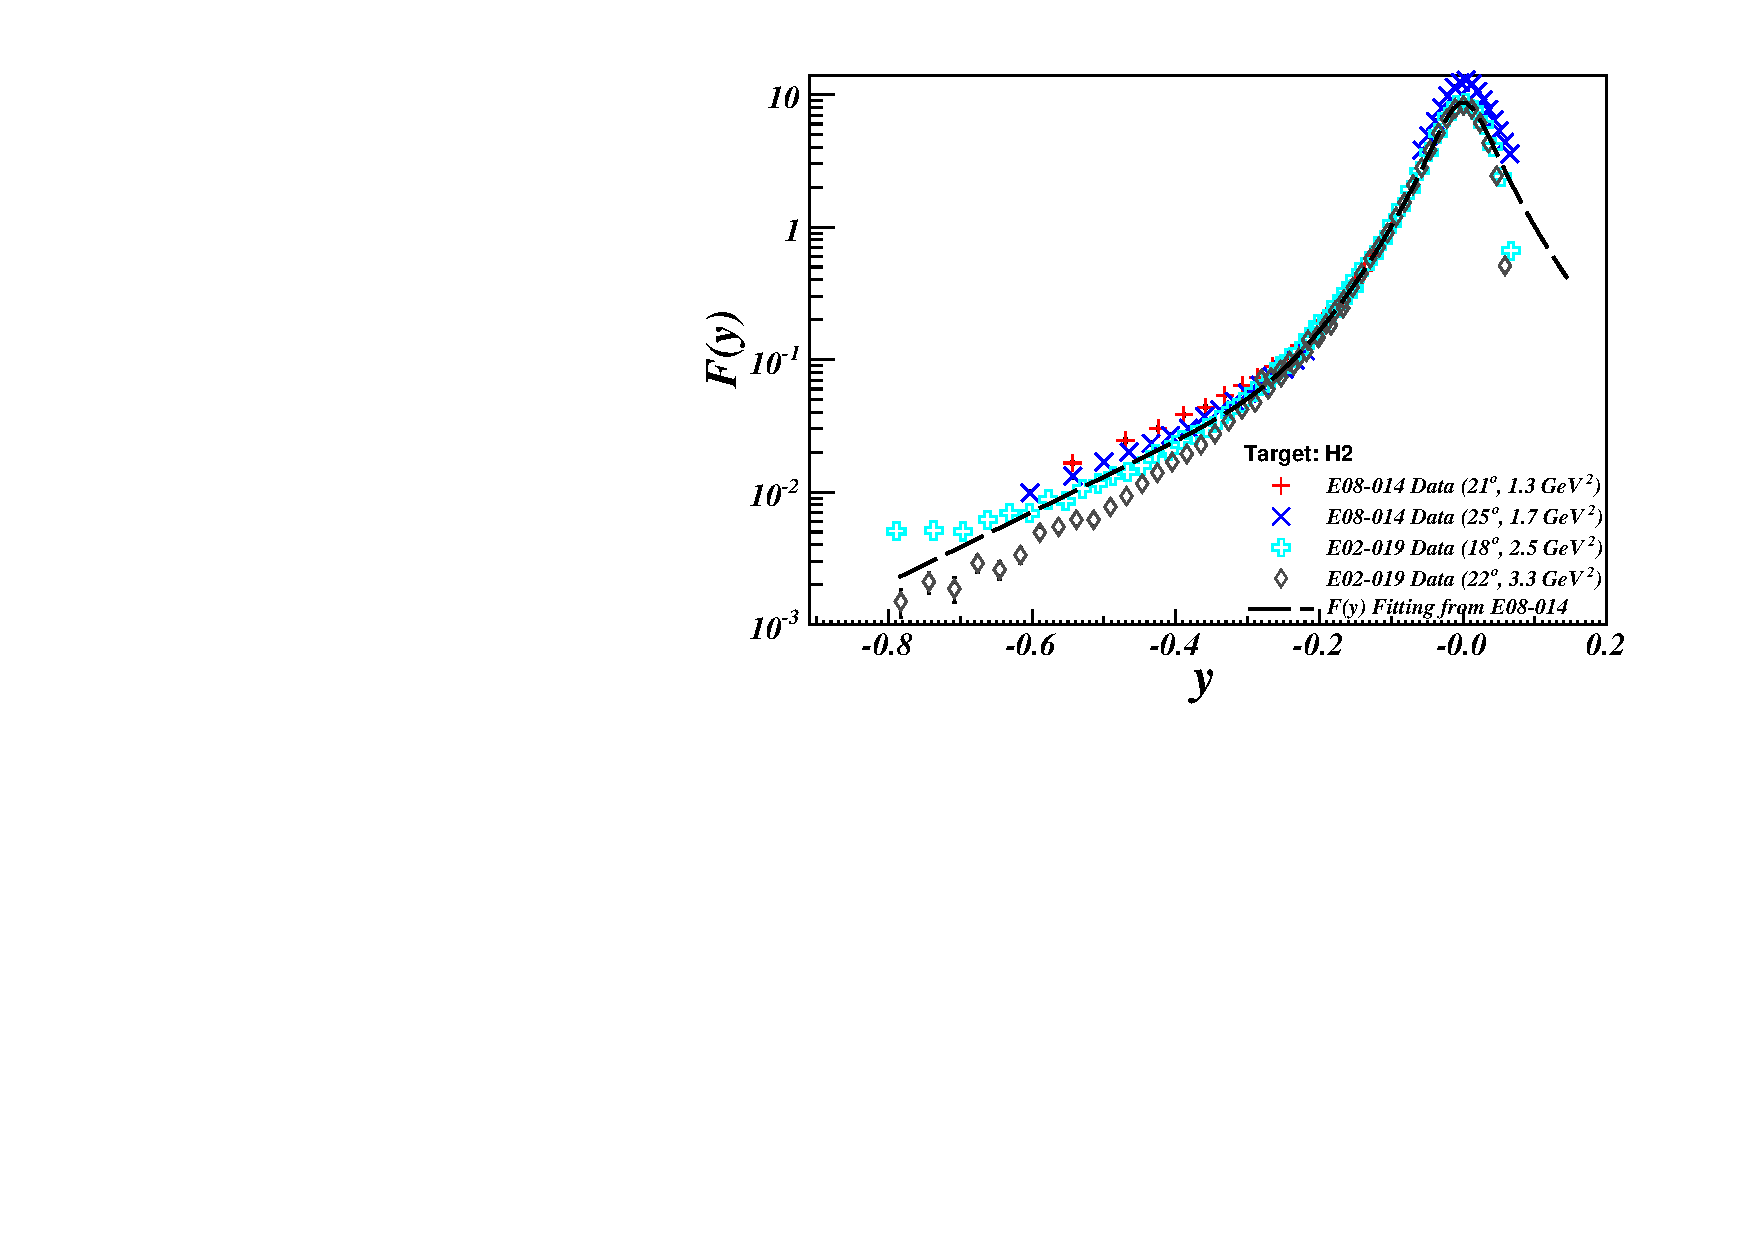
\includegraphics[type=pdf,ext=.pdf,read=.pdf,width=.90\textwidth]{./figures/xs/H2_XGT2_Fy}
    \caption[$F(y)$ distribution for $\mathrm{^{2}H}$]{\footnotesize{$F(y)$ distribution for $\mathrm{^{2}H}$. Symbols are experimental results from the E08-014 and the E02-019, where the kinematic settings are as indicated. The dash line is the fit of the new data with Eq.~\eqref{fy_fit_func1}. The new results have better agreement with the lowest $\mathrm{Q^{2}}$ data from the E02-019 at $18^{\circ}$ and deviate from the $22^{\circ}$ data with a higher $\mathrm{Q^{2}}$ value. It could be due to the FSI contribution. At $y\simeq 0$, the $25^{\circ}$ data significantly deviates from the E02-019 results, which might be due to the difference DIS subtraction procedure.}}
    \label{fy_h2_xgt2}
  \end{center}
\end{figure}
 \begin{figure}[!ht]
  \begin{center}
    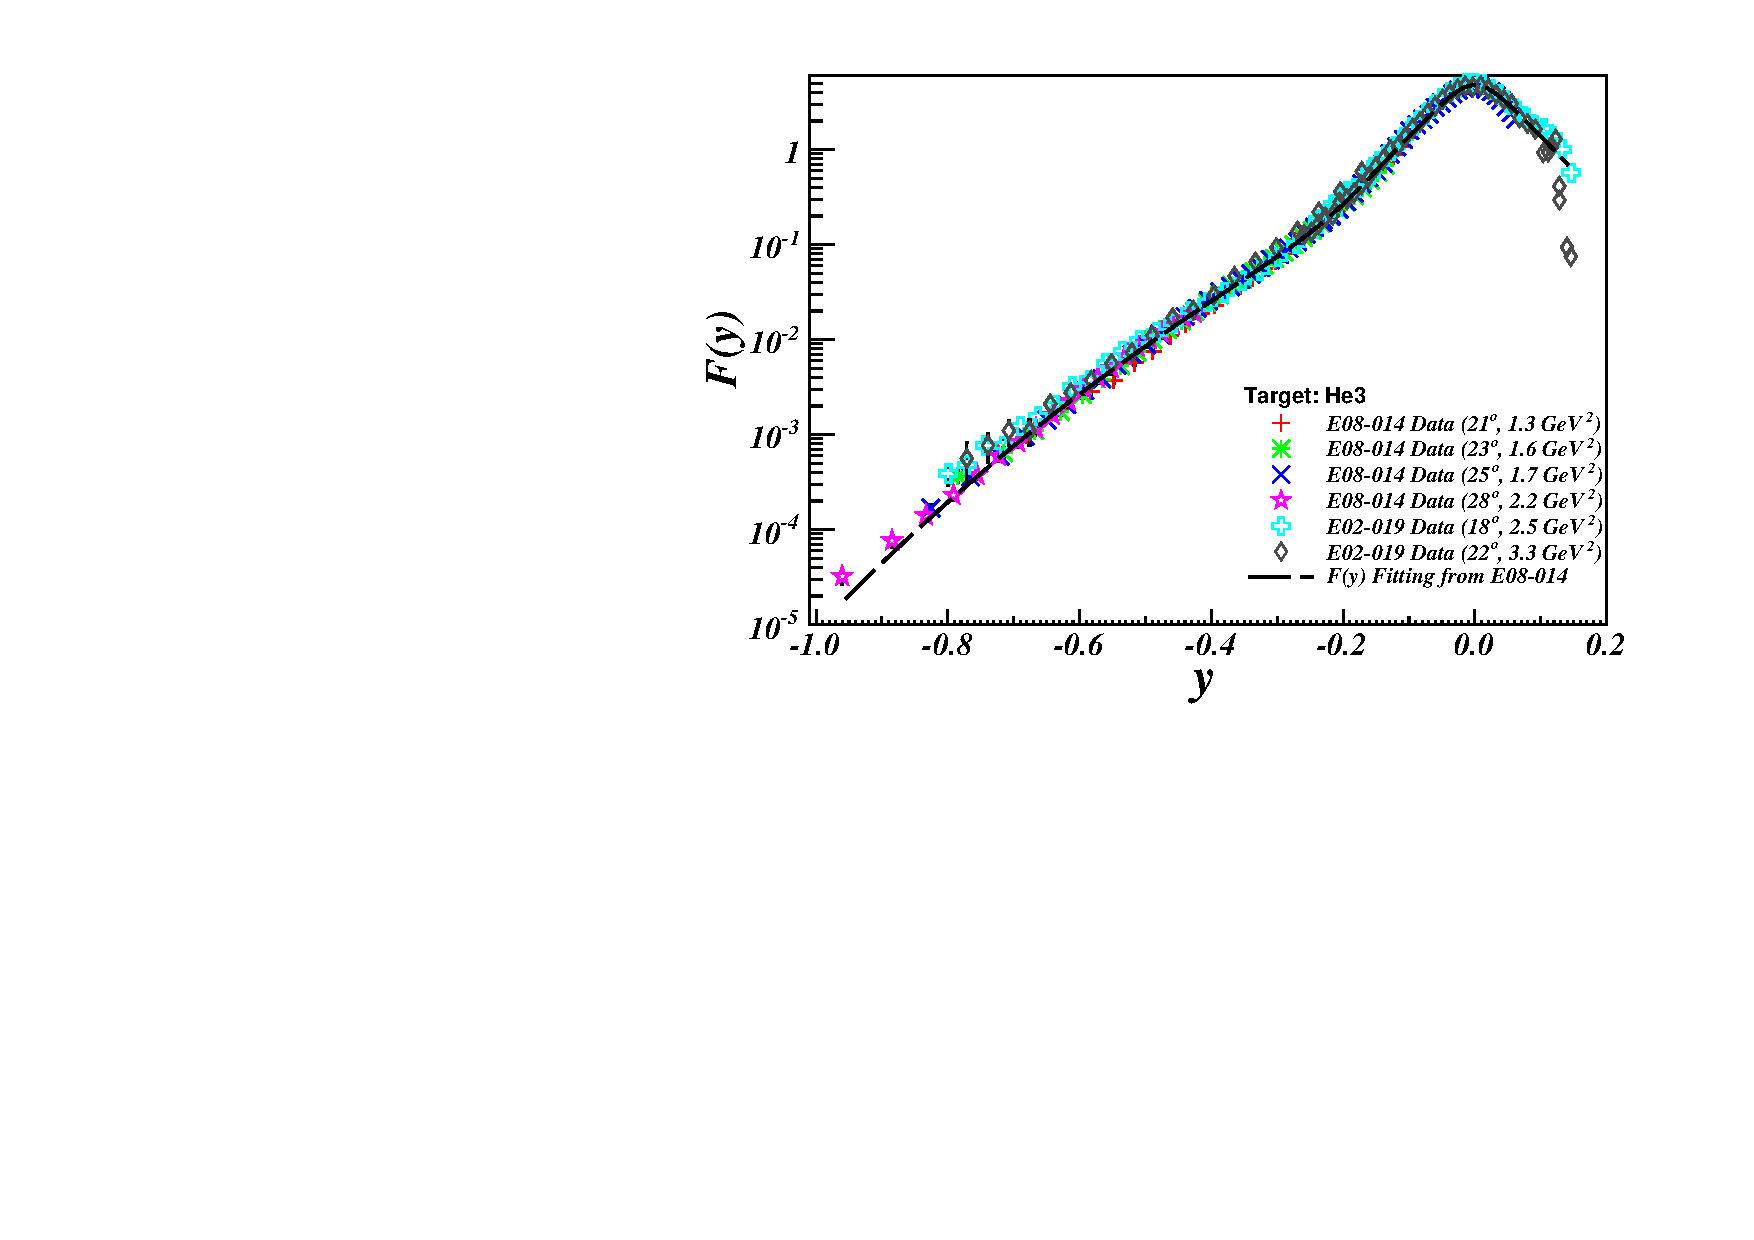
\includegraphics[type=pdf,ext=.pdf,read=.pdf,width=.90\textwidth]{./figures/xs/He3_XGT2_Fy}
    \caption[$F(y)$ distribution for $\mathrm{^{3}He}$]{\footnotesize{$F(y)$ distribution for $\mathrm{^{3}He}$. Symbols are experimental results from the E08-014 and the E02-019, where the kinematic settings are as indicated. The dash line is the fit of the new data with Eq.~\eqref{fy_fit_func2}.}}
    \label{fy_he3_xgt2}
  \end{center}
\end{figure}
 \begin{figure}[!ht]
  \begin{center}
    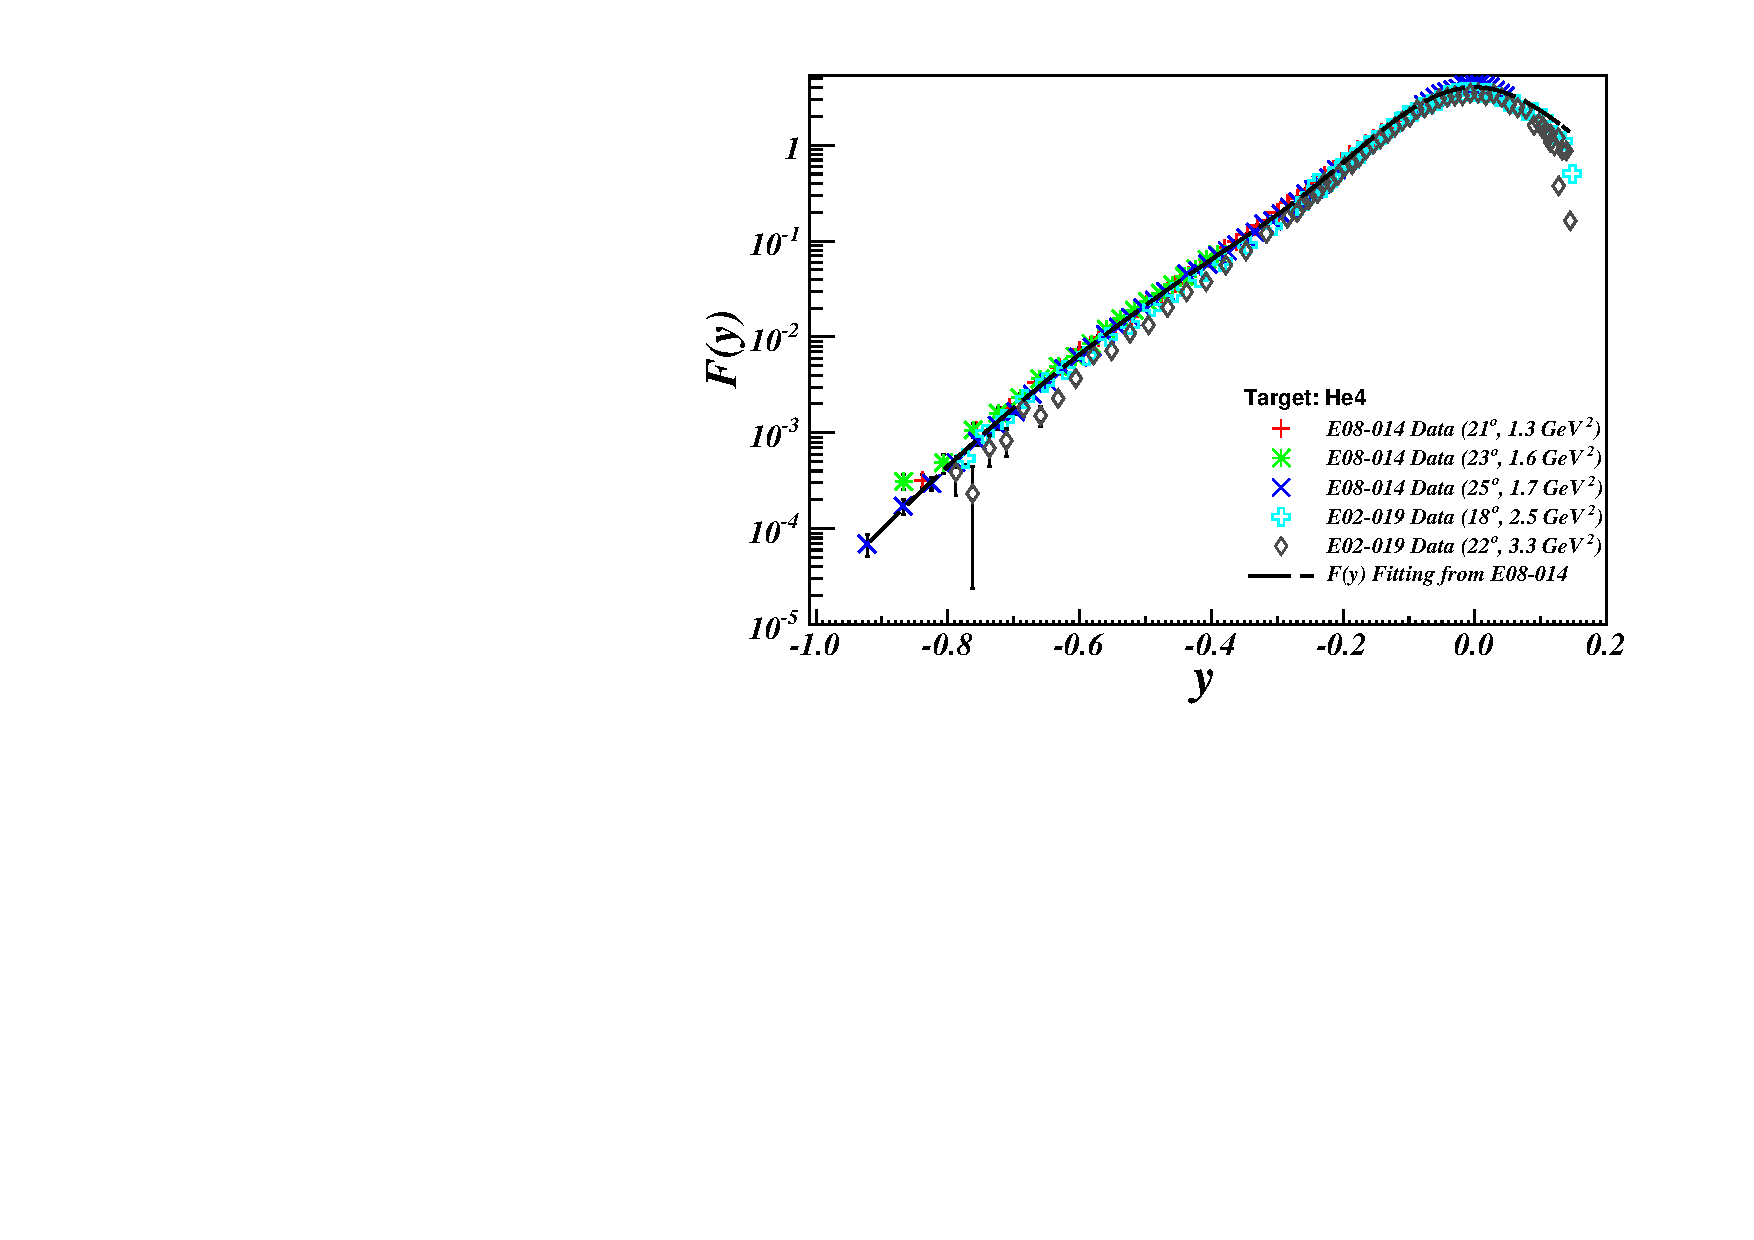
\includegraphics[type=pdf,ext=.pdf,read=.pdf,width=.90\textwidth]{./figures/xs/He4_XGT2_Fy}
    \caption[$F(y)$ distribution for $\mathrm{^{4}He}$]{\footnotesize{$F(y)$ distribution for $\mathrm{^{4}He}$. Symbols are experimental results from the E08-014 and the E02-019, where the kinematic settings are as indicated. The dash line is the fit of the new data with Eq.~\eqref{fy_fit_func2}.}}
    \label{fy_he4_xgt2}
  \end{center}
\end{figure}
\begin{figure}[!ht]
  \begin{center}
    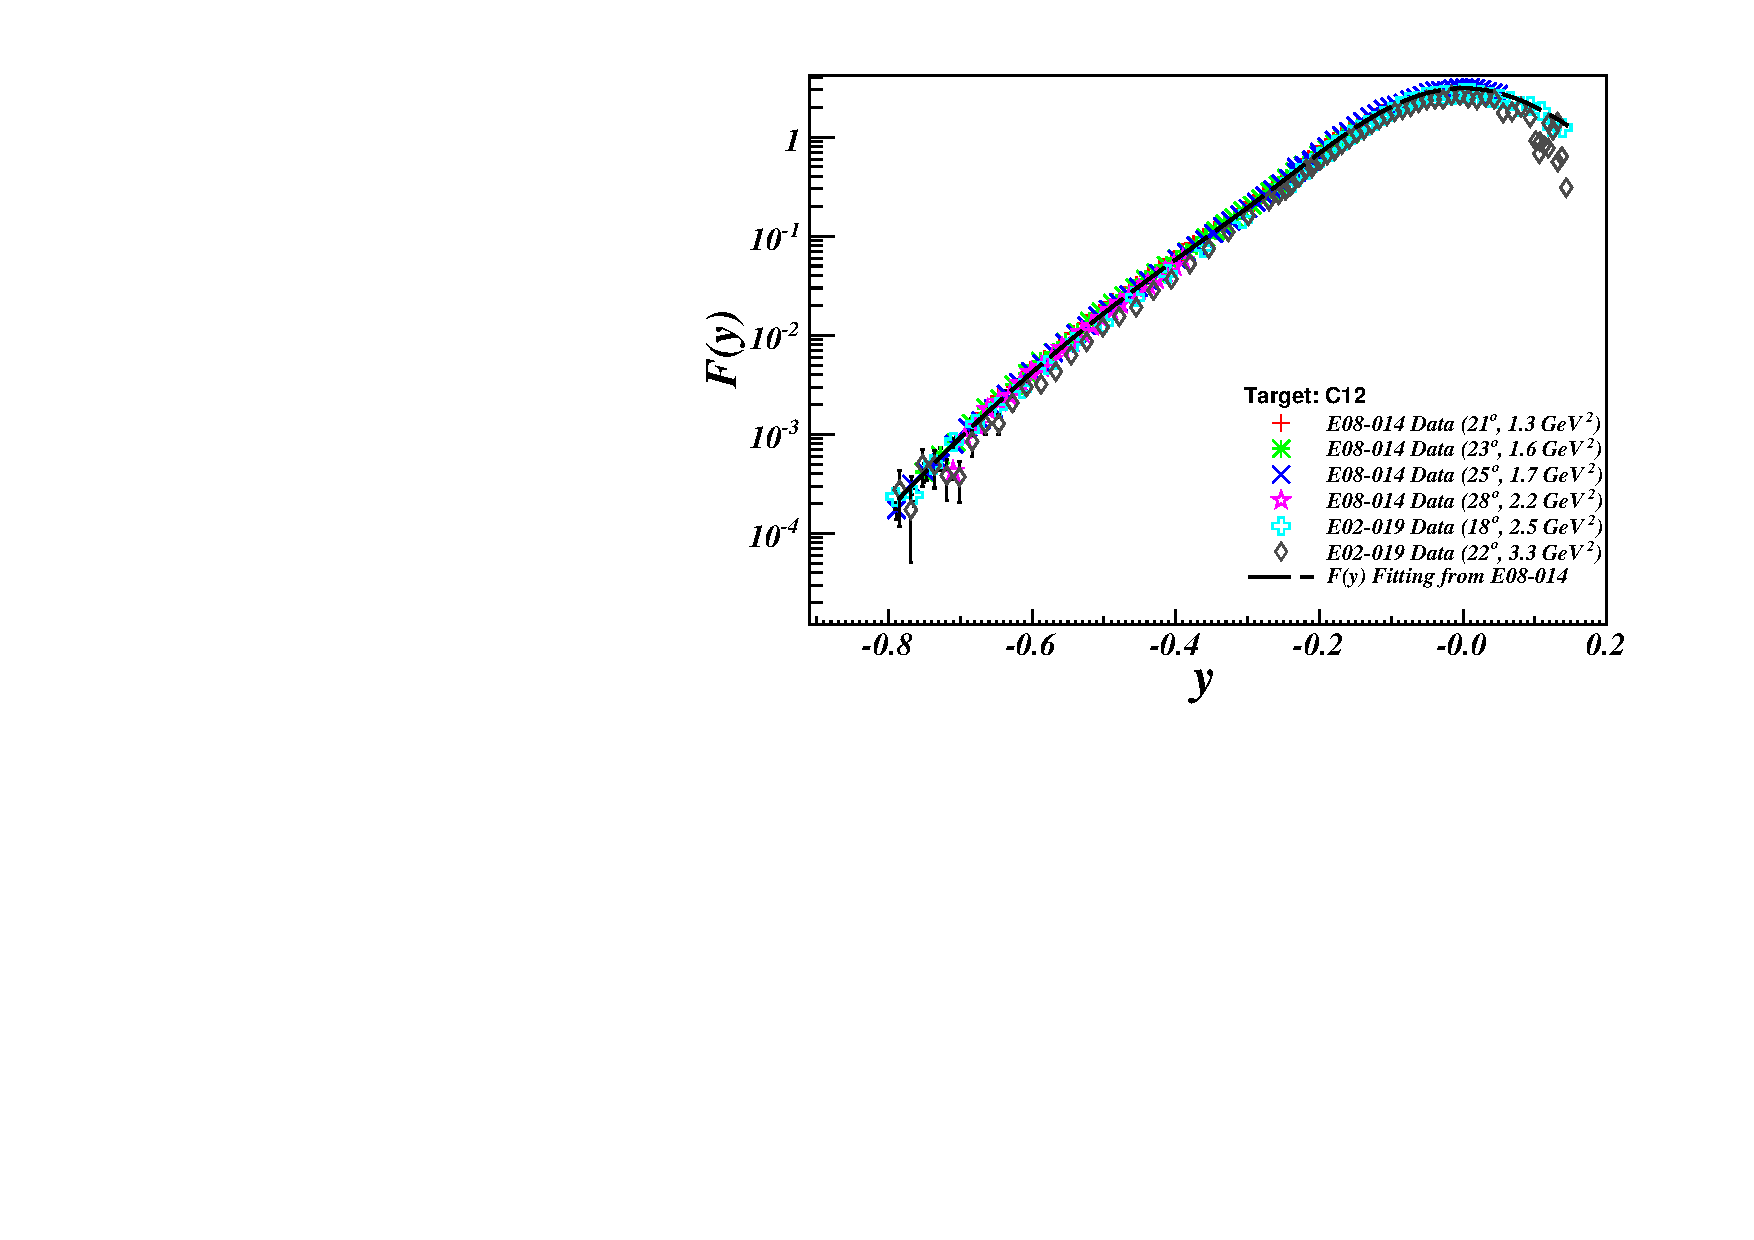
\includegraphics[type=pdf,ext=.pdf,read=.pdf,width=.90\textwidth]{./figures/xs/C12_XGT2_Fy}
    \caption[$F(y)$ distribution for $\mathrm{^{12}C}$]{\footnotesize{$F(y)$ distribution for $\mathrm{^{12}C}$. Symbols are experimental results from the E08-014 and the E02-019, where the kinematic settings are as indicated. The dash line is the fit of the new data with Eq.~\eqref{fy_fit_func2}.}}
    \label{fy_c12_xgt2}
  \end{center}
\end{figure}
 \begin{figure}[!ht]
  \begin{center}
    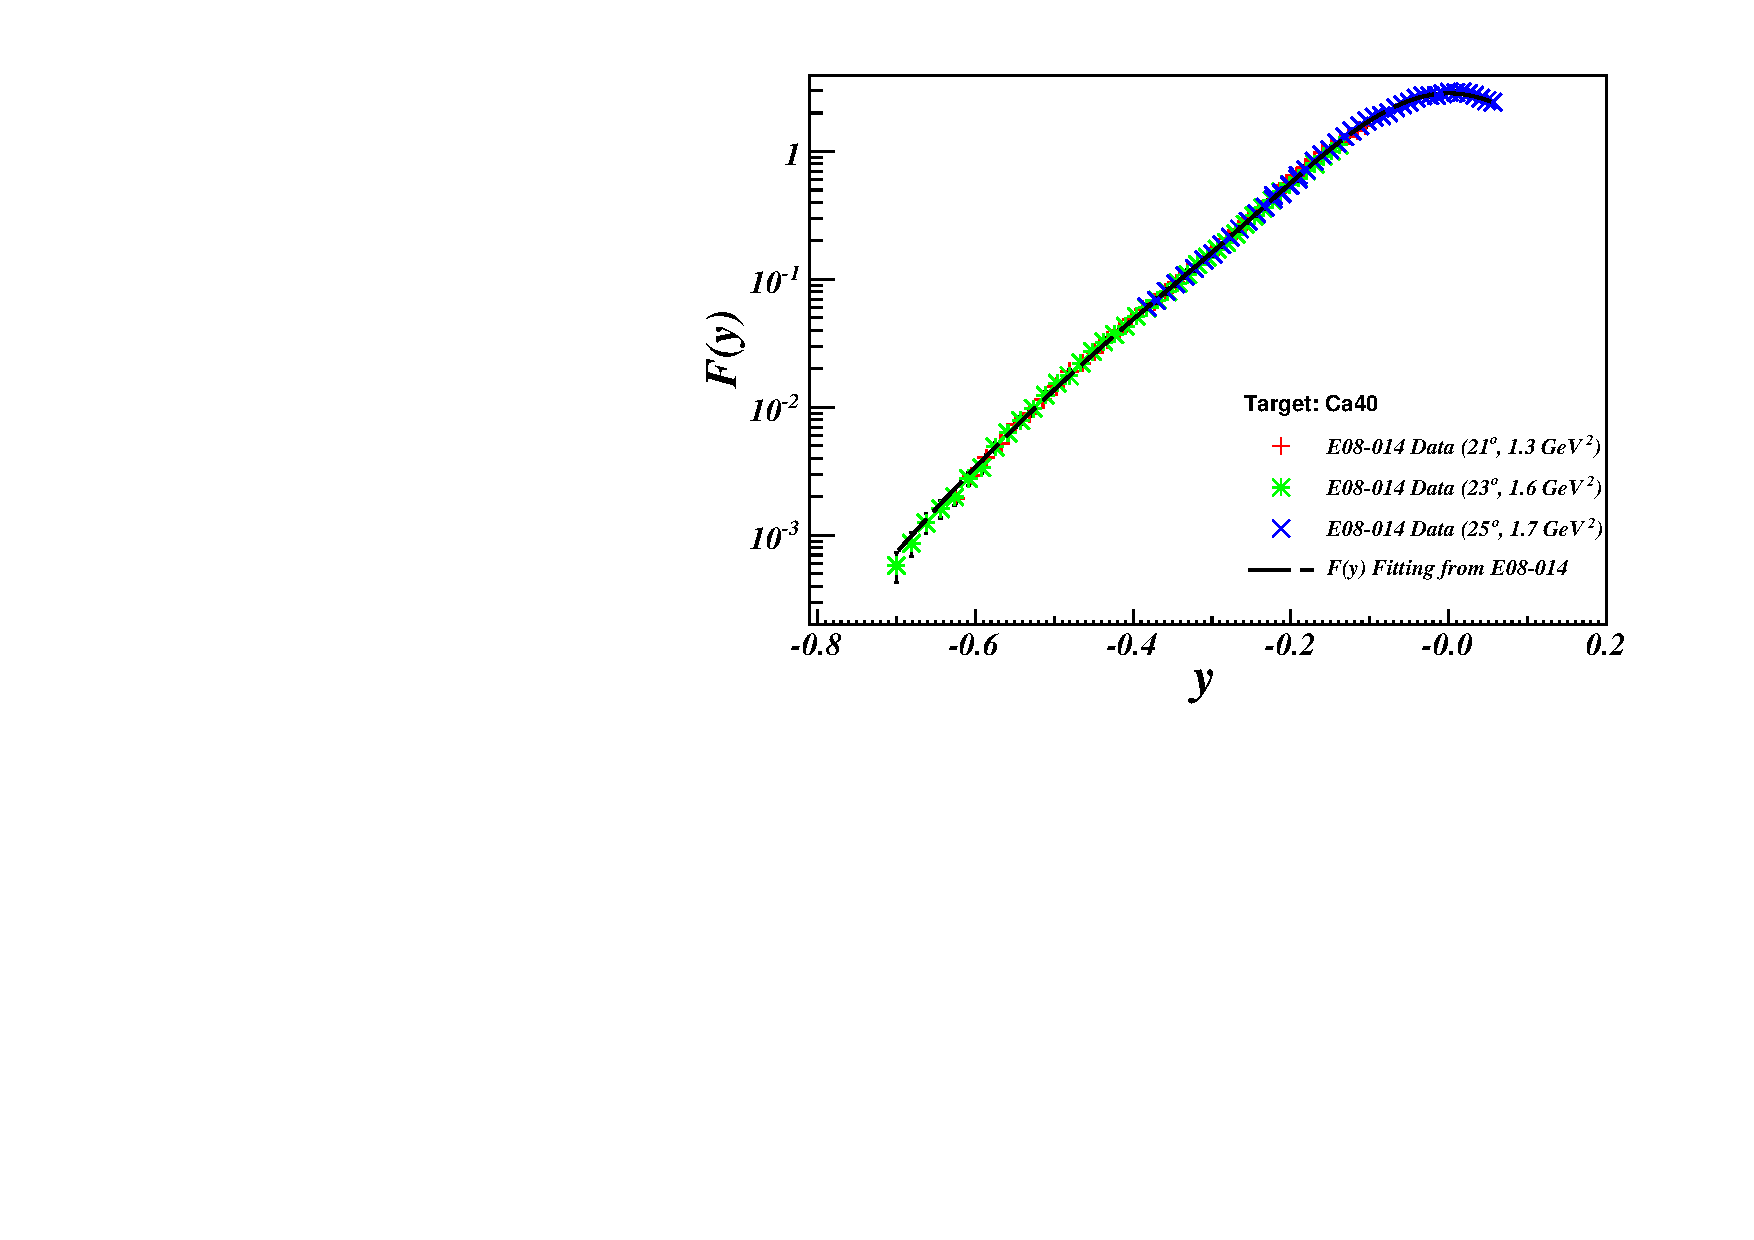
\includegraphics[type=pdf,ext=.pdf,read=.pdf,width=.90\textwidth]{./figures/xs/Ca40_XGT2_Fy}
    \caption[$F(y)$ distribution for $\mathrm{^{40}Ca}$]{\footnotesize{$F(y)$ distribution for $\mathrm{^{40}C}$. Symbols are experimental results from the E08-014, where the kinematic settings are as indicated. The dash line is the fit of the new data with Eq.~\eqref{fy_fit_func2}.}}
    \label{fy_ca40_xgt2}
  \end{center}
\end{figure}
 \begin{figure}[!ht]
  \begin{center}
    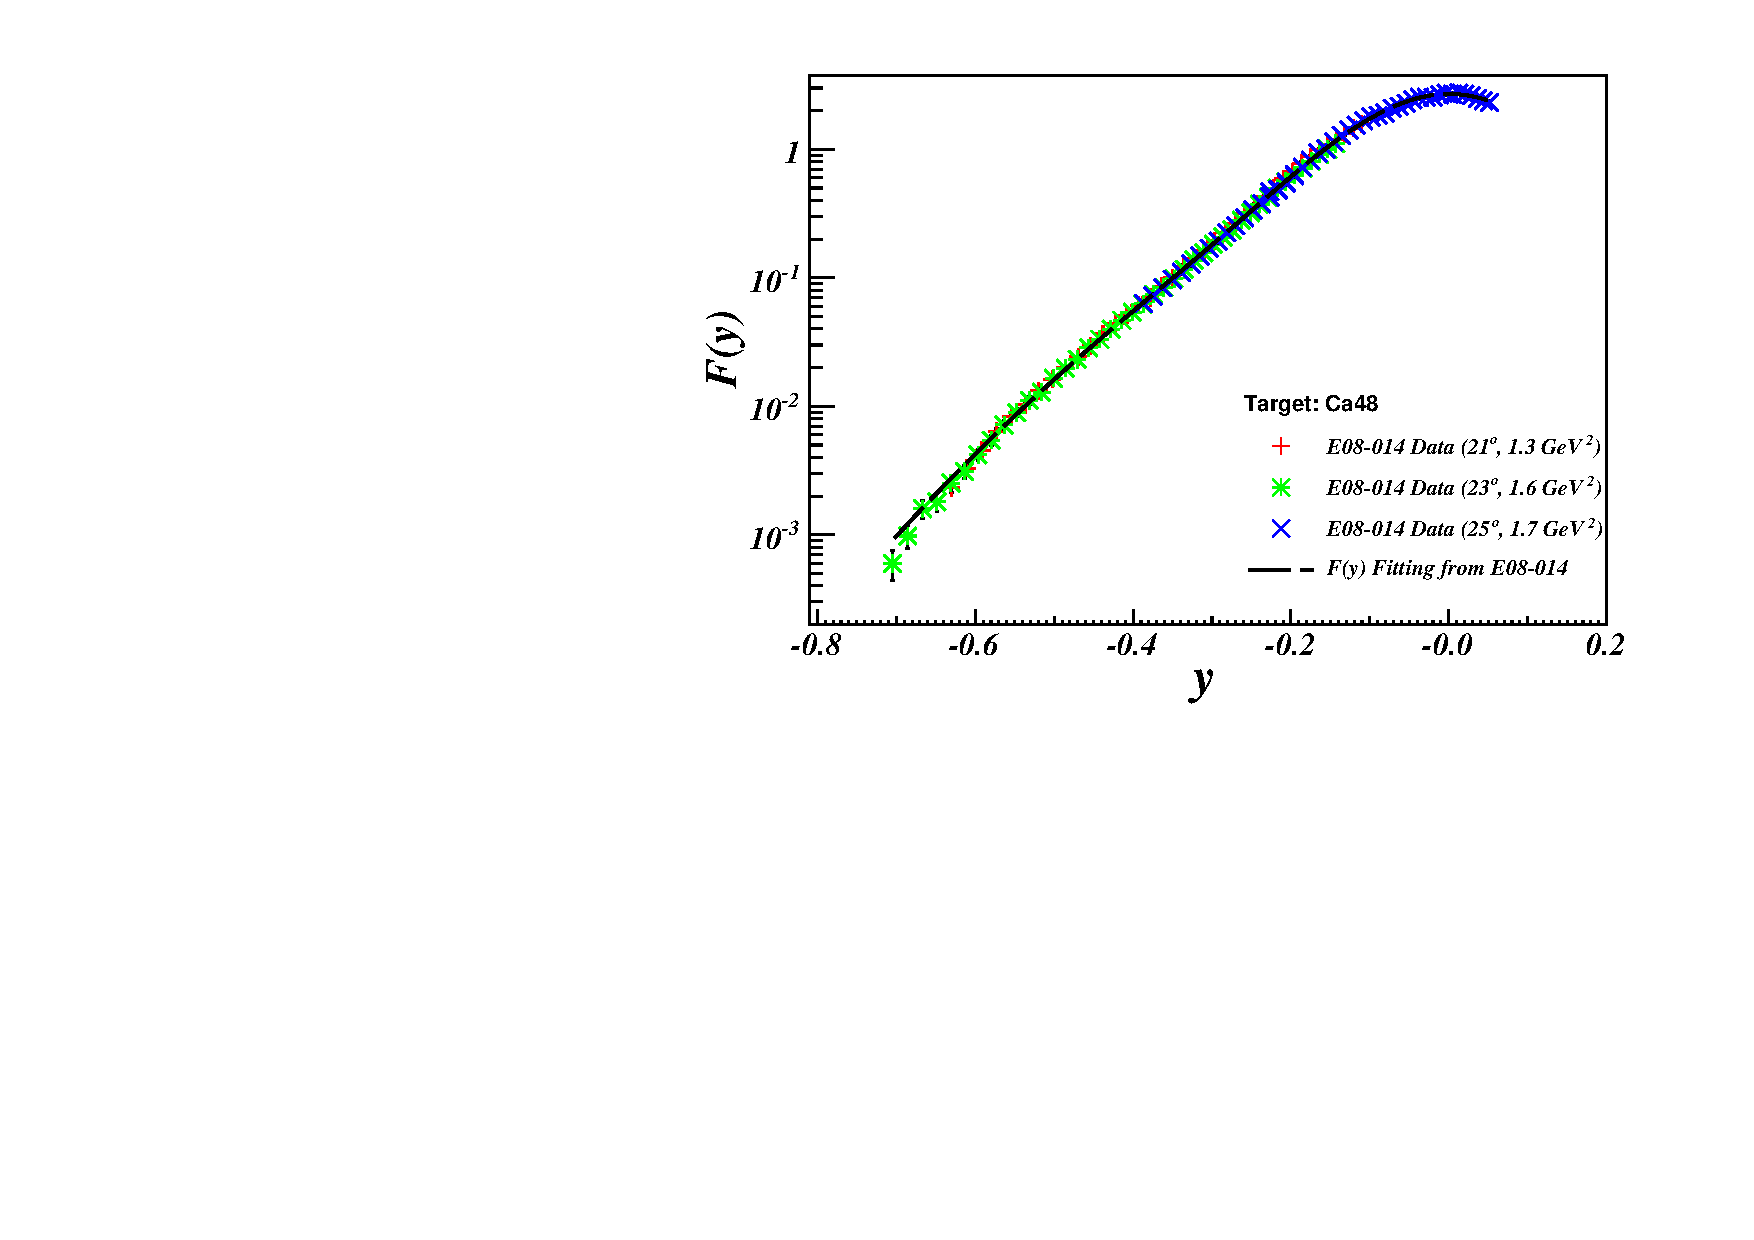
\includegraphics[type=pdf,ext=.pdf,read=.pdf,width=.90\textwidth]{./figures/xs/Ca48_XGT2_Fy}
    \caption[$F(y)$ distribution for $\mathrm{^{48}Ca}$]{\footnotesize{$F(y)$ distribution for $\mathrm{^{48}C}$ extracted from the experimental cross sections. Symbols are experimental results from the E08-014, where the kinematic settings are indicated. The dash line is the fit of the new data with Eq.~\eqref{fy_fit_func2}.}}
    \label{fy_ca48_xgt2}
  \end{center}
\end{figure}
  As discussed in Section 1.2.2, the y-scaling function, $F(y)$, is one of the most important features of Quasielastic scattering (QE) and it can be applied to extract the momentum distribution of the nucleus. $F(y)$ can be obtained from the experimental cross sections with Eq.~\eqref{fy_scaling_eq2}, after removing the deep inelastic scattering (DIS) contributions. 
   
  The $F(y)$ distributions for $\mathrm{^{2}H}$, $\mathrm{^{3}He}$, $\mathrm{^{4}He}$, $\mathrm{^{12}C}$, $\mathrm{^{40}Ca}$ and $\mathrm{^{48}Ca}$ were extracted from the preliminary cross section results given in Appendix E, and they are presented in Fig.~\ref{fy_h2_xgt2}, Fig.~\ref{fy_he3_xgt2}, Fig.~\ref{fy_he4_xgt2}, Fig.~\ref{fy_c12_xgt2}, Fig.~\ref{fy_ca40_xgt2}, and Fig.~\ref{fy_ca48_xgt2}, respectively. The E02-019 data from Hall-C with larger $\mathrm{Q^{2}}$ was also compared with each target, except $\mathrm{^{40}Ca}$ and $\mathrm{^{48}Ca}$ which were firstly measured in this experiment with high $\mathrm{Q^{2}}$.
  
   From these plots, the distributions at different $\mathrm{Q^{2}}$ tend to be nearly identical and generally show very small $Q^{2}$ dependence. The only significant $\mathrm{Q^{2}}$ dependence occurs for deuterium at $y<-0.4~GeV/c$ where there is a clear decrease in $F(y)$ with $\mathrm{Q^{2}}$, as shown in Fig.~\ref{fy_h2_xgt2}. Also in this plot, one notices that at $y\simeq 0$ where the QE peak locates, there is a non-trivial disagreement between the new data at $25^{\circ}$ and the E02-19 data. This might be due to the different DIS subtraction procedures. As mentioned in Section 1.2.2, a cross section model is required to remove the DIS contributions from the experimental cross sections, and two different models were used for these two experiments.
 
 As also shown in these plots, the extracted $F(y)$ distributions for all $\mathrm{Q^{2}}$ settings were fitted with the fitting function, Eq.~\eqref{fy_fit_func1} for deuteron and Eq.~\eqref{fy_fit_func2} for other heavier nuclei, as given in Appendix II.

 The momentum distribution for each nucleus was also extracted from the fit of the new results with Eq.~\eqref{mom_dis_fy}. The distributions for different nuclei are compared in Fig.~\ref{mom_dis_xgt2}. The absolute strength of each nucleus is comparable with the one given in Fig.~\ref{mom_dis_ox}. As discussed in Chapter 2, the momentum distributions for different nuclei should have similar shapes for $k>k_{F}$ due to the short-distance property of the 2N-SRC pairs in nuclei. The results given in Fig.~\ref{mom_dis_xgt2} show identical curves at high momentum ($k>300~MeV/c$). 
   \begin{figure}[!ht]
  \begin{center}
    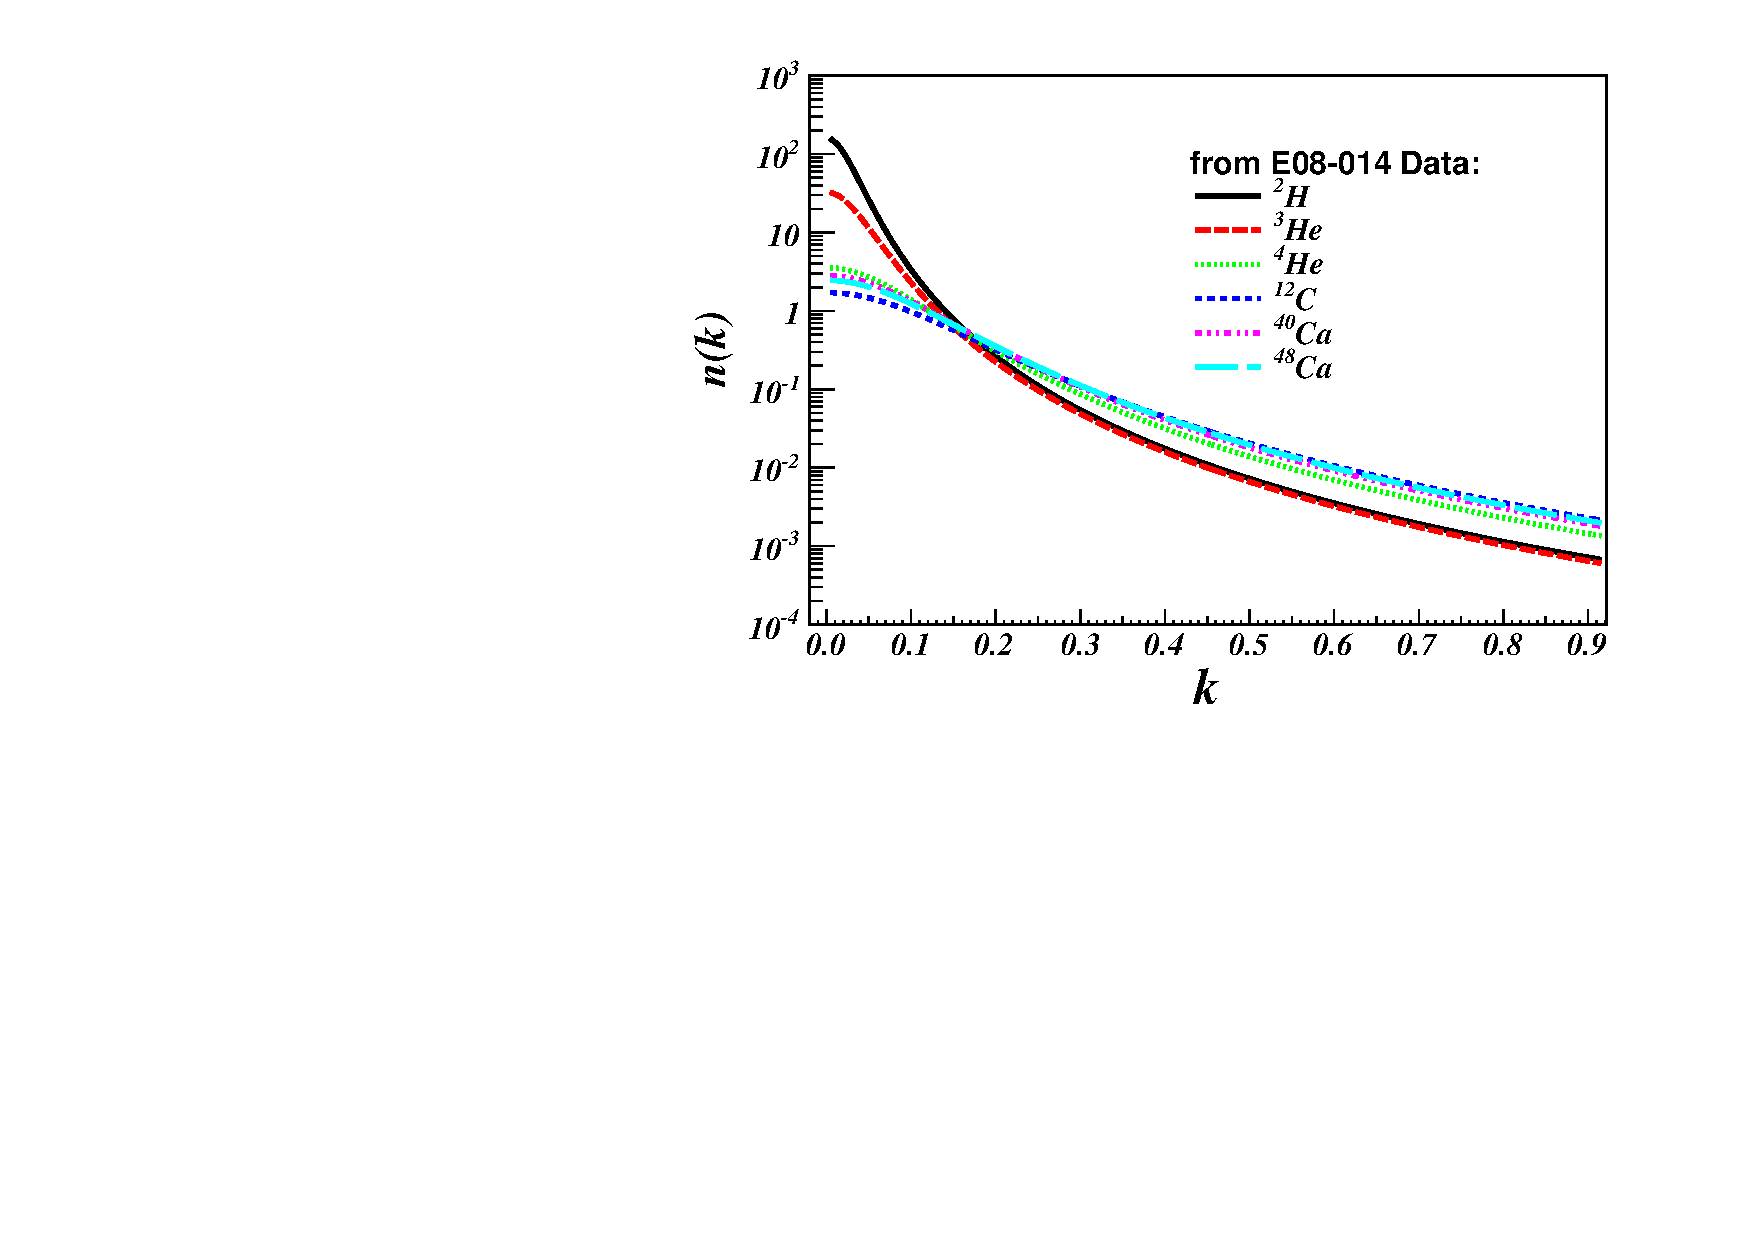
\includegraphics[type=pdf,ext=.pdf,read=.pdf,width=1.\textwidth]{./figures/xs/Mom_Dis_XGT2}
    \caption[Momentum distribution for all nuclei]{\footnotesize{Momentum distribution for all nuclei, where the distributions were extracted from the $F(y)$ function fitted from the experimental cross sections.}}
    \label{mom_dis_xgt2}
  \end{center}
\end{figure}

\section{2N-SRC and 3N-SRC Ratios}
\subsection{$\mathrm{^{4}He/^{3}He}$}
 \begin{figure}[!ht]
  \begin{center}
    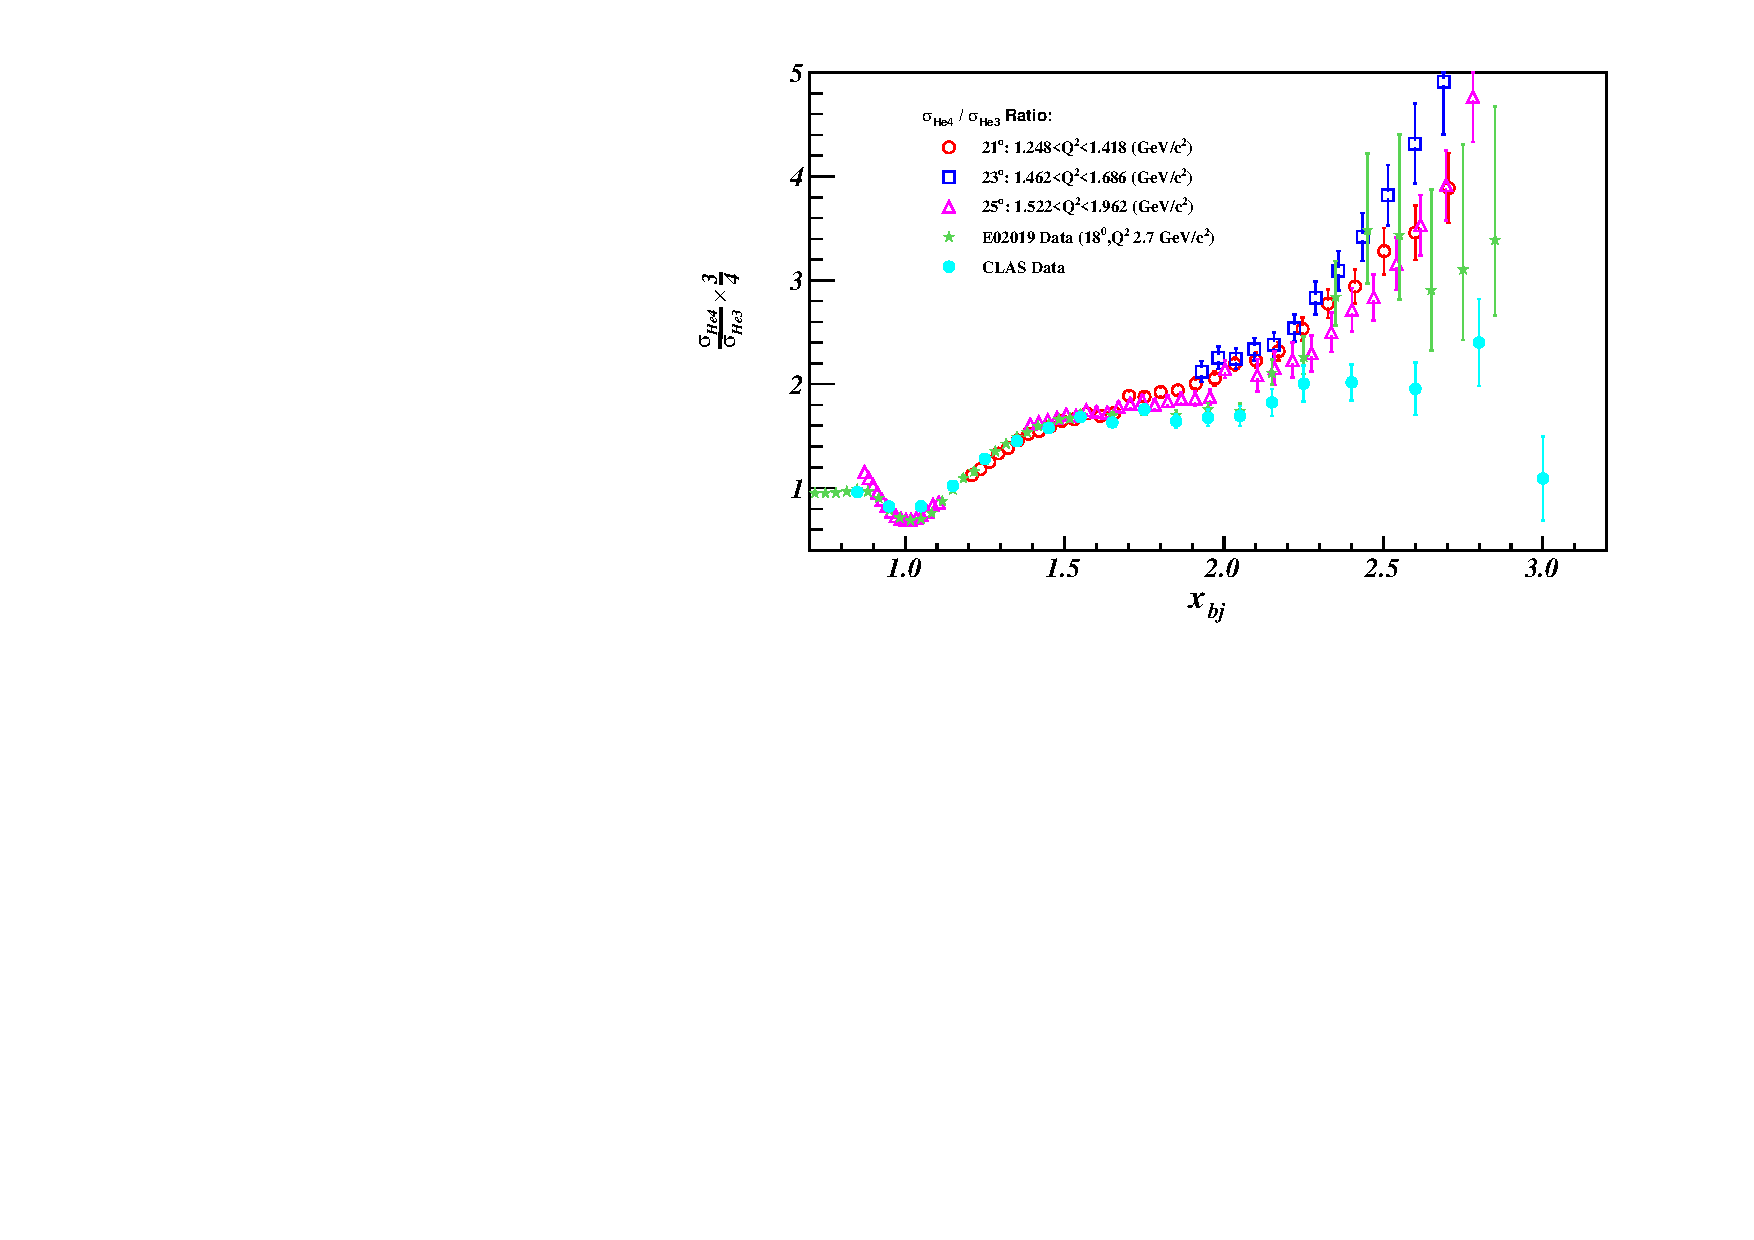
\includegraphics[type=pdf,ext=.pdf,read=.pdf,width=0.95\textwidth]{./figures/xs/He4_He3_XS_Ratio_Zoom}
    \caption[Cross section ratio of $\mathrm{^{4}He}$ to $\mathrm{^{3}He}$]{\footnotesize{Cross section ratio of $\mathrm{^{4}He}$ to $\mathrm{^{3}He}$. Open symbols are the new E08-14 data at $21^{\circ}$ (circle), $23^{\circ}$ (box), and $25^{\circ}$ (triangle). The values of the 2N-SRC ratio from the E02-019 data~\cite{PhysRevLett.108.092502} (solid boxes) at $18^{\circ}$ and CLAS data~\cite{PhysRevLett.96.082501} (solid dishes) are also included from comparison.}}
    \label{ratio_he4_he3}
  \end{center}
\end{figure}
 The preliminary cross section ratio of $\mathrm{^{4}He}$ to $\mathrm{^{3}He}$ is given in Fig.~\ref{ratio_he4_he3}. In the 2N-SRC region ($1.3<x_{bj}<2$), the $21^{\circ}$ data does not reveal a plateau. It is consistent with the CLAS data~\cite{PhysRevLett.96.082501} which found a breakdown of the plateau below $\mathrm{Q^{2}=1.4~GeV^{2}}$. The $\mathrm{^{4}He}$ data at $23^{\circ}$ does not cover the 2N-SRC region. However, the $25^{\circ}$ data does show an obvious plateau in the 2N-SRC region and a fit in $1.55<x_{bj}<1.85$ gives the value of the plateau equal to 1.84$\pm$0.01. Within the same $x_{bj}$ range, the CLAS data gives the plateau at 1.68$\pm$0.02, and the value in the E02-019 data~\cite{PhysRevLett.108.092502} is 1.71$\pm$ 0.02 at $18^{\circ}$. The result from CLAS agrees more with the one from the E02-019, while the preliminary result of this experiment is about 8\% larger. The new data was taken at lower $\mathrm{Q^{2}}$ compared with the E02-019 data, but the CLAS data was taken at the similar $\mathrm{Q^{2}}$ range, so the reason for the disagreement is yet unknown. The E02-019 data has been corrected for the Coulomb effect, and this correction will also be applied to this data later.
 
  In the 3N-SRC region for $x_{bj}>2$, this new data tends to agree with the E02-019 data. Neither data sets reveal a flat region starting from $x_{bj}\simeq 2.3$ as seen in the CLAS data. While the E02-019 result has large error bars in this region, the new data has much smaller error bars. However, one can not draw a firm conclusion from the current results, and more detailed analysis work for the new data must be completed before the results are final.
 
 \subsection{$\mathrm{^{12}C/^{3}He}$}
 \begin{figure}[!ht]
  \begin{center}
    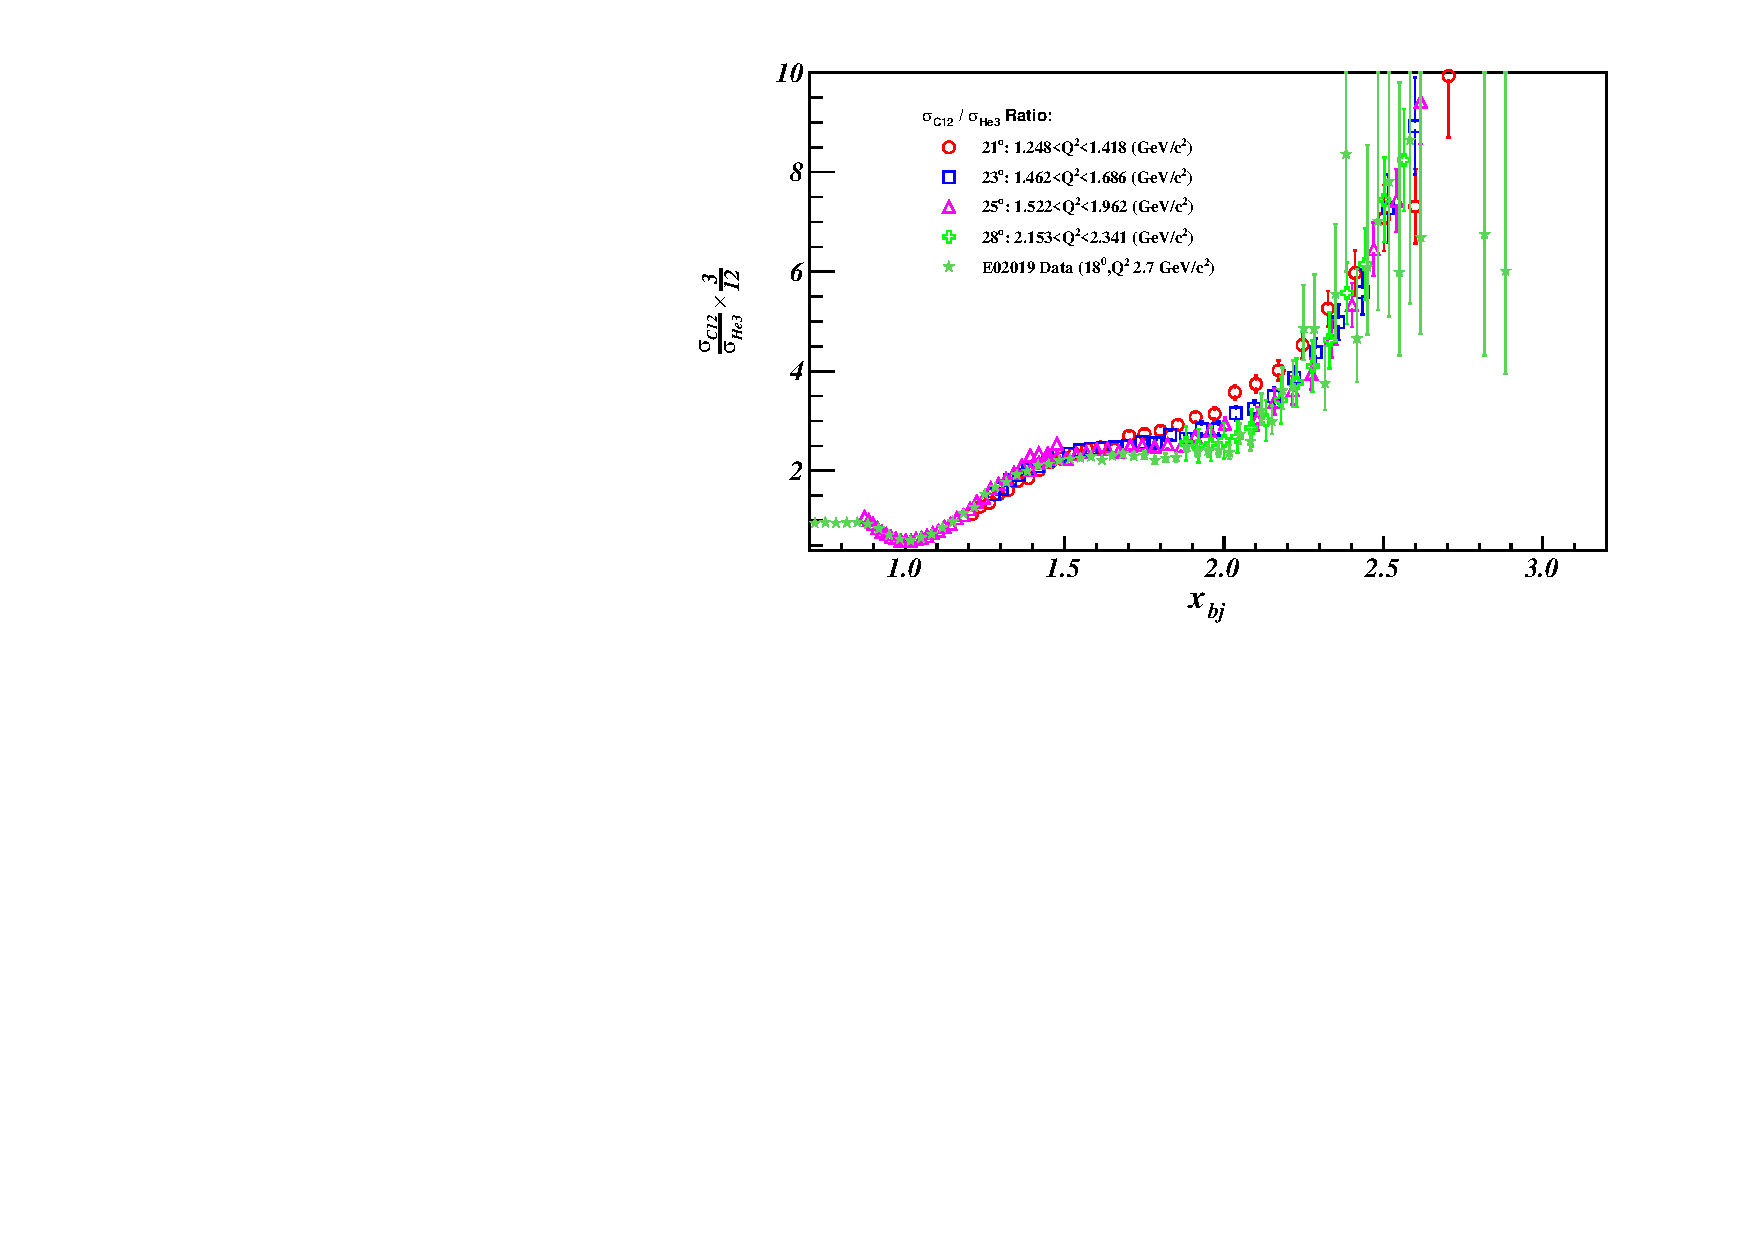
\includegraphics[type=pdf,ext=.pdf,read=.pdf,width=1.\textwidth]{./figures/xs/C12_He3_XS_Ratio_Zoom}
    \caption[Cross section ratio of $\mathrm{^{12}C}$ to $\mathrm{^{3}He}$]{\footnotesize{Cross section ratio of $\mathrm{^{12}C}$ to $\mathrm{^{3}He}$, compared with the E02-019 preliminary results. Open symbols are the new E08-14 data at $21^{\circ}$ (circle), $23^{\circ}$ (box), $25^{\circ}$ (triangle) and $28^{\circ}$ (), respectively. The solid boxes are the E02-019 data. The $\mathrm{Q^{2}}$ value for each setting is given in the plot.}}
    \label{ratio_c12_he3}
  \end{center}
\end{figure}
Fig.~\ref{ratio_c12_he3} shows the preliminary cross section ratio of $\mathrm{^{12}C}$ to $\mathrm{^{3}He}$, as well as the results from the E02-019 data. Overall, both experiments have a good agreement in the region of the 2N-SRC, and the new result does not indicate a plateau of the 3N-SRC for $x_{bj}>2$.

 For each kinematic setting, a linear fit was performed for $1.55<x_{bj}<1.85$ to extract the ratio in the 2N-SRC region. For the E08-014 data, the values of the 2N-SRC plateau at $21^{\circ}$, $23^{\circ}$ and $25^{\circ}$  are 2.60$\pm$0.01, 2.46$\pm$0.01 and 2.43$\pm$0.01, respectively. For the E02-019 data, the value is 2.27$\pm$0.02. The 2N-SRC ratio decreases with increasing $\mathrm{Q^{2}}$, which suggests that FSI may still play an important role in these kinematic regions. 

\subsection{$\mathrm{^{40}Ca/^{2}H}$ and $\mathrm{^{48}Ca/^{2}H}$}
The 2N-SRC plateaus of the Calcium isotopes were firstly measured in this experiment, as shown in Fig.~\ref{ca40_h2_xgt2} and Fig.~\ref{ca48_h2_xgt2}. The values of $a_{2}$ for $\mathrm{^{40}Ca}$ and $\mathrm{^{48}Ca}$ are 4.987$\pm$0.018 and 4.863$\pm$0.016, respectively.  
 \begin{figure}[!ht]
  \begin{center}
    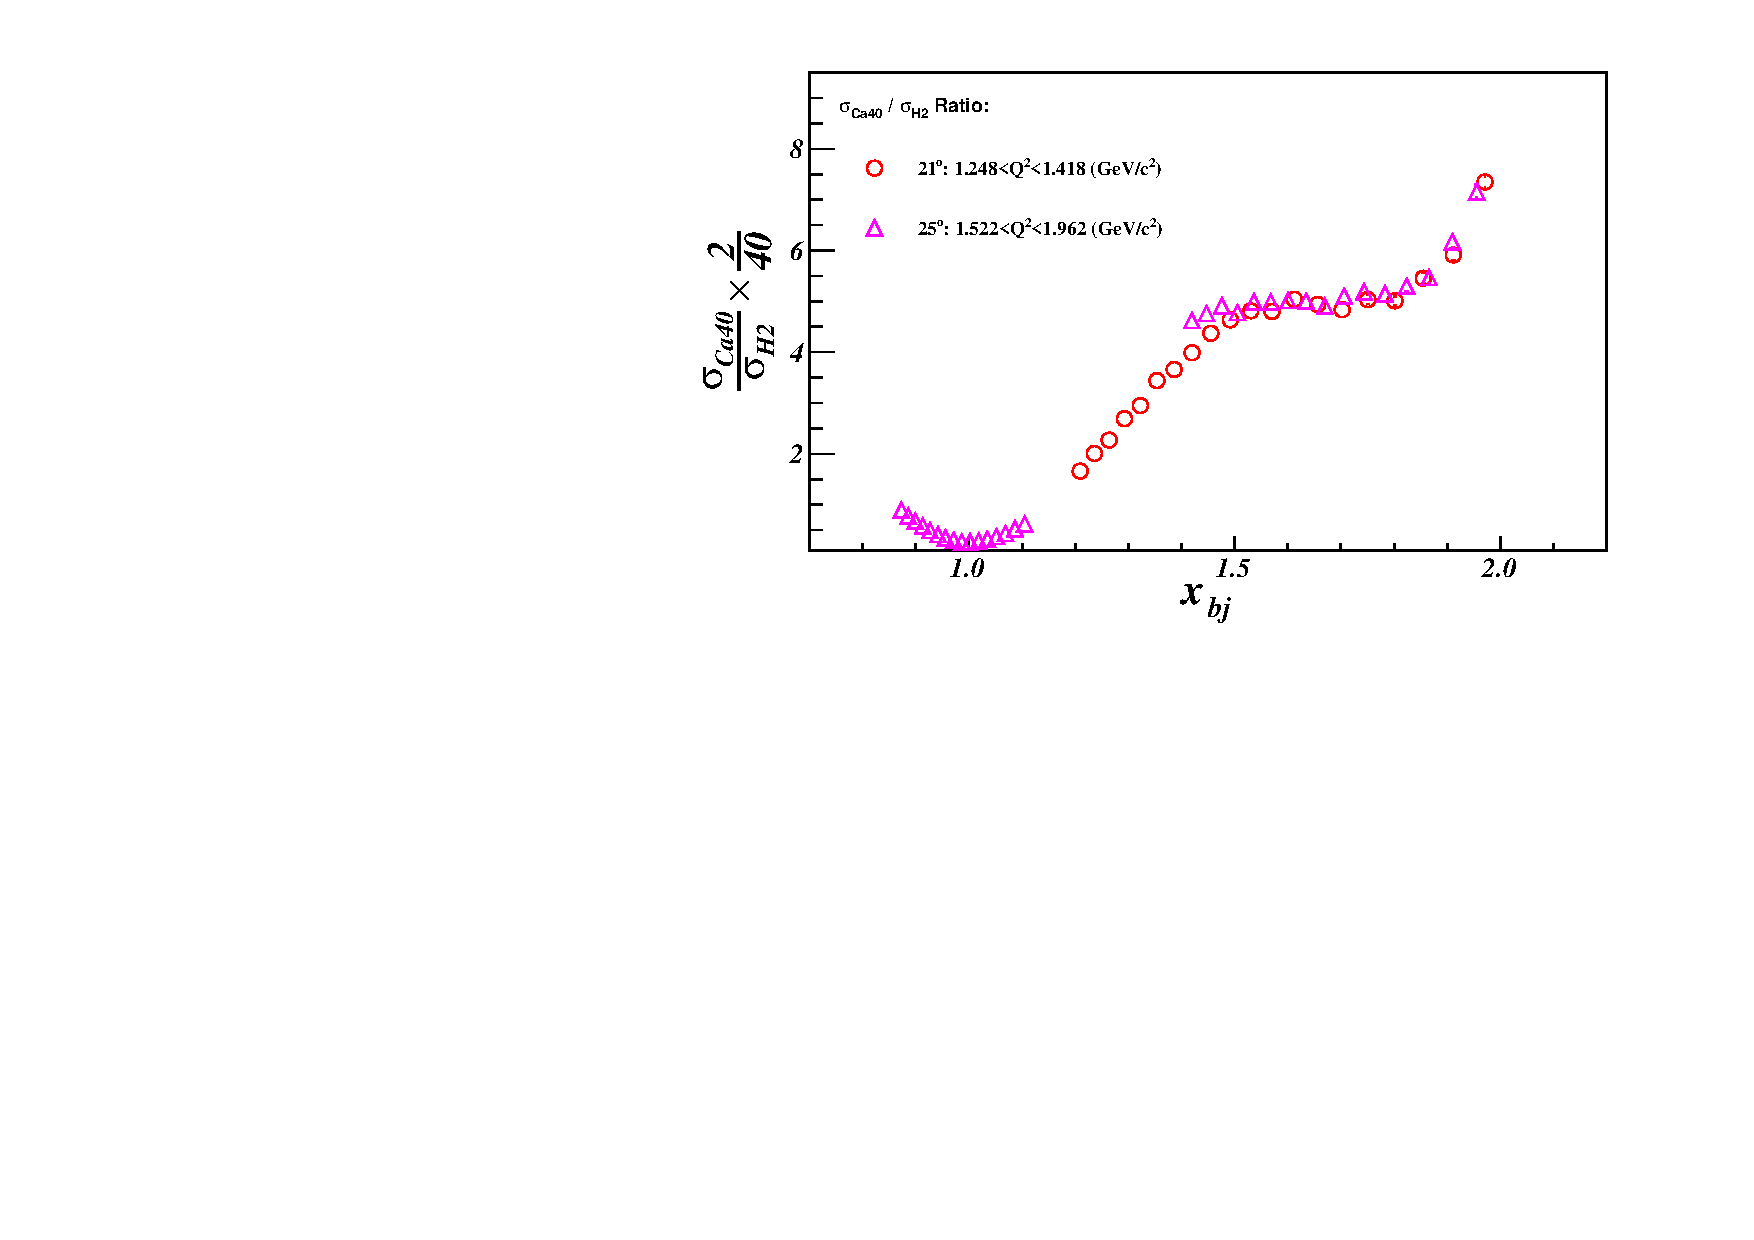
\includegraphics[type=pdf,ext=.pdf,read=.pdf,width=0.9\textwidth]{./figures/xs/Ca40_H2_XS_Ratio}
   \caption[Cross section ratios of $\mathrm{^{40}Ca}$ to $\mathrm{^{2}H}$]{\footnotesize{Cross section ratios of $\mathrm{^{40}Ca}$ to $\mathrm{^{2}H}$.}}
    \label{ca40_h2_xgt2}
  \end{center}
\end{figure}
\begin{figure}[!ht]
  \begin{center}
    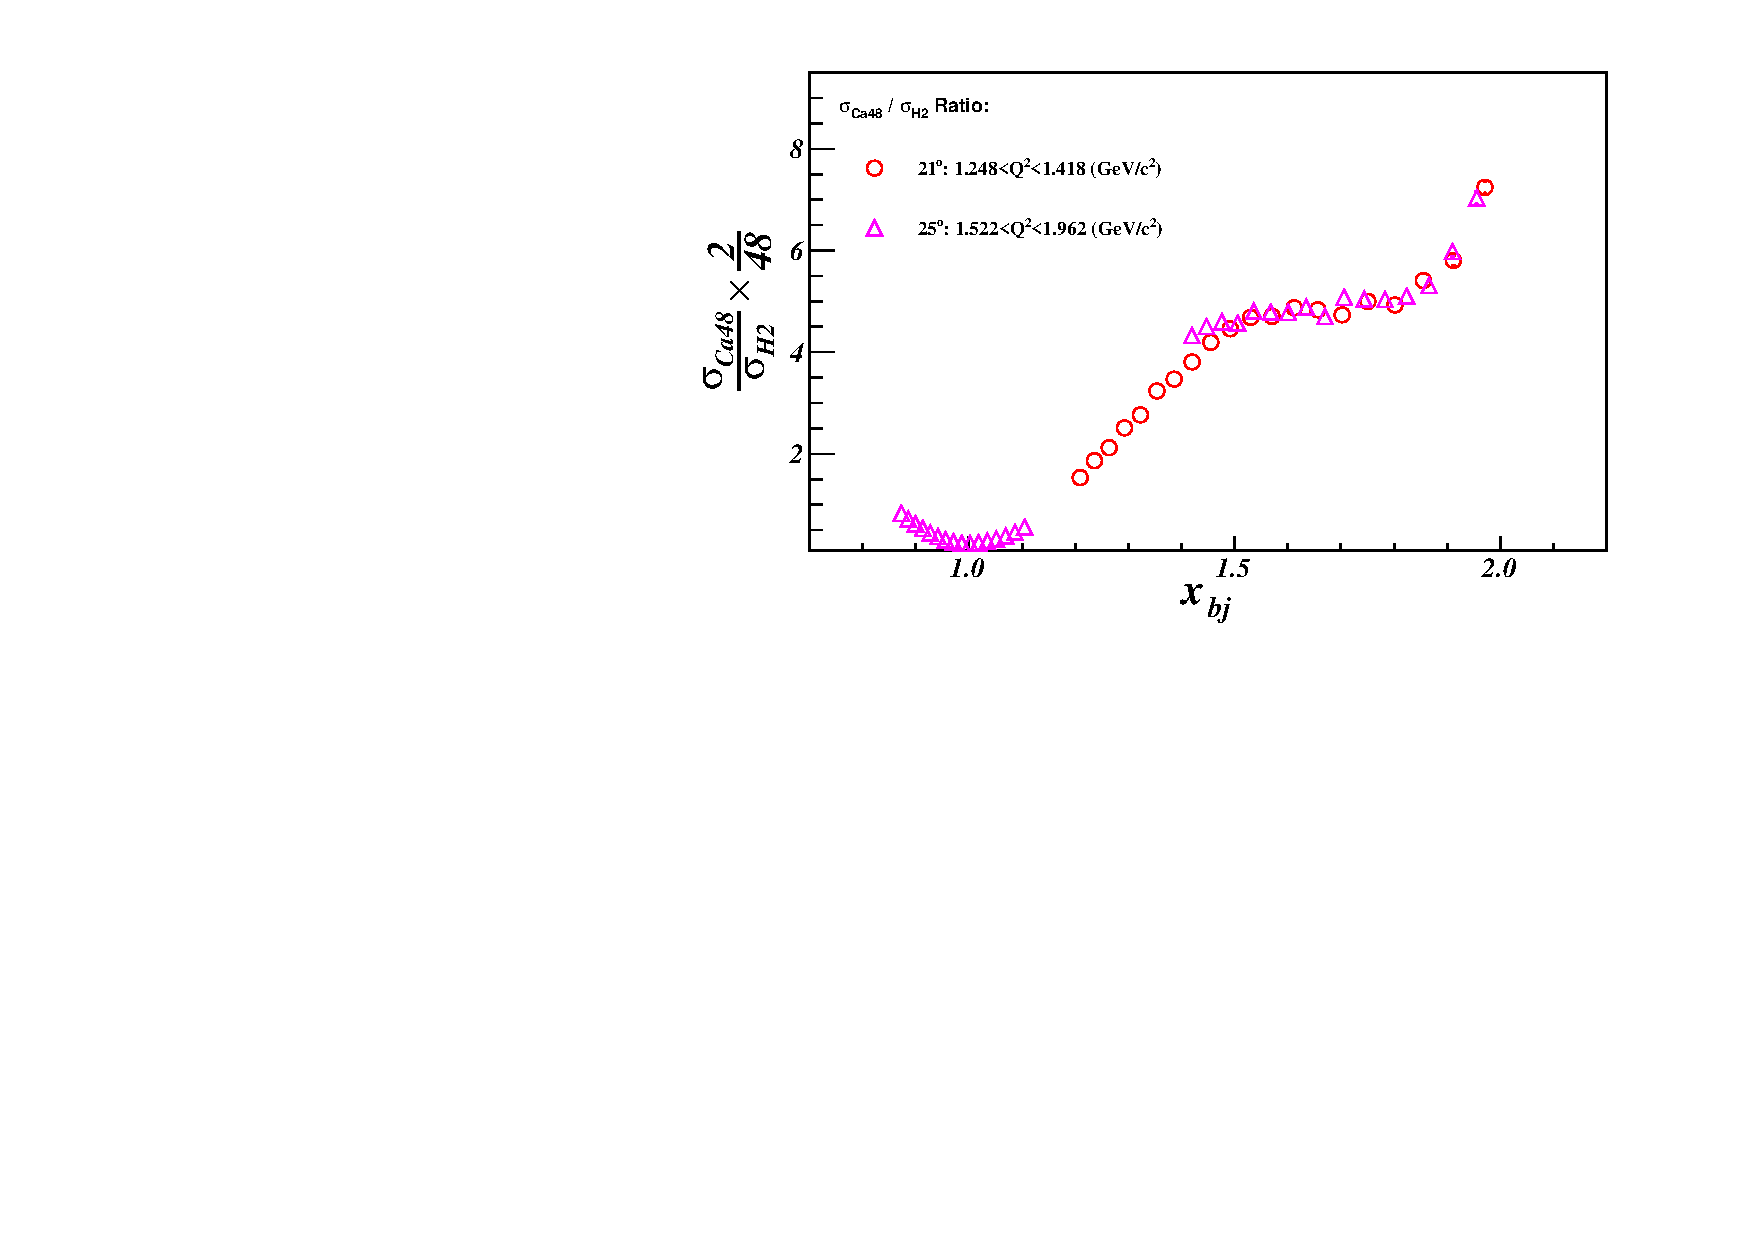
\includegraphics[type=pdf,ext=.pdf,read=.pdf,width=0.9\textwidth]{./figures/xs/Ca48_H2_XS_Ratio}
   \caption[Cross section ratios of $\mathrm{^{48}Ca}$ to $\mathrm{^{2}H}$]{\footnotesize{Cross section ratios of $\mathrm{^{48}Ca}$ to $\mathrm{^{2}H}$.}}
    \label{ca48_h2_xgt2}
  \end{center}
\end{figure}
\begin{figure}[!ht]
  \begin{center}
    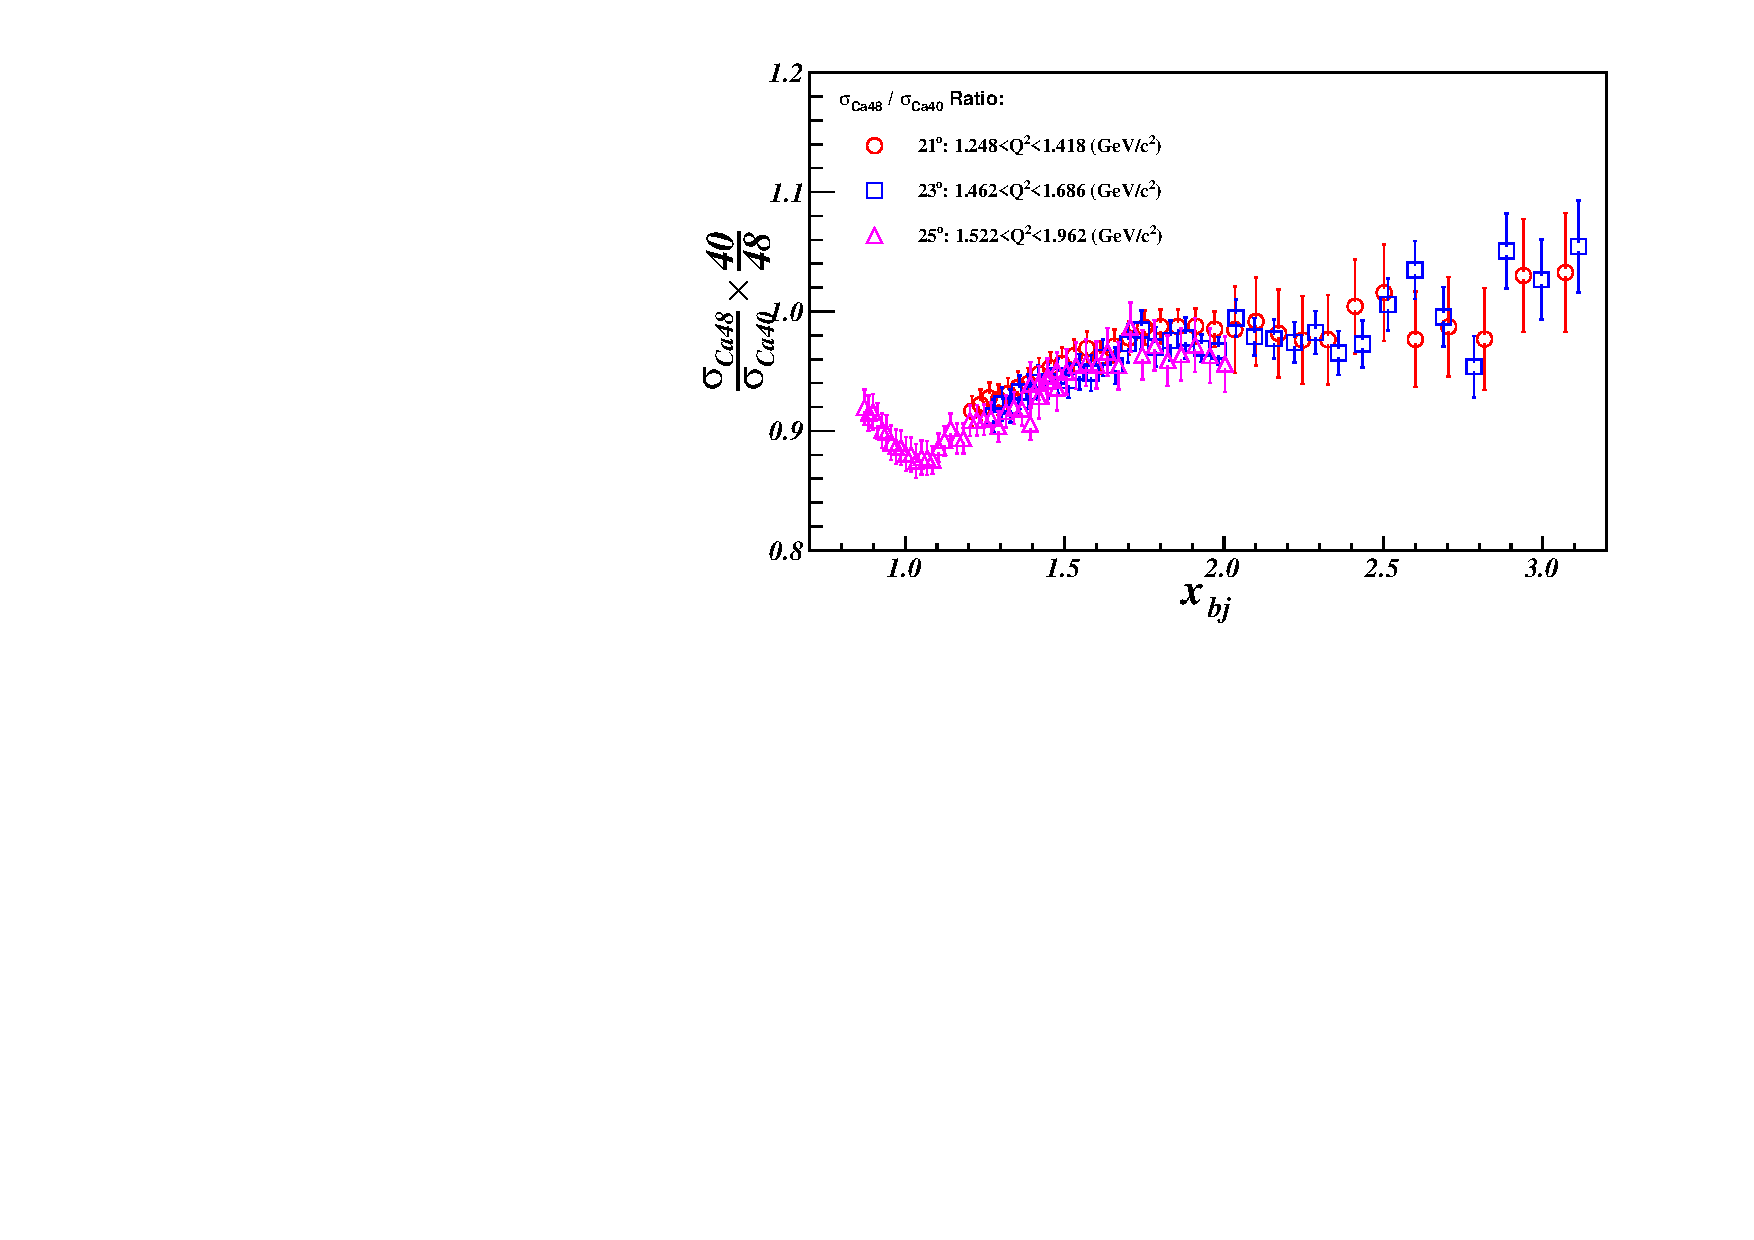
\includegraphics[type=pdf,ext=.pdf,read=.pdf,width=1.\textwidth]{./figures/xs/Ca48_Ca40_XS_Ratio}
    \caption[Cross section ratio of $\mathrm{^{48}Ca}$ to $\mathrm{^{40}Ca}$]{\footnotesize{Cross section ratio of $\mathrm{^{48}Ca}$ to $\mathrm{^{40}Ca}$}}
    \label{ratio_ca48_ca40}
  \end{center}
\end{figure}
\section{Isospin Effect Study with $\mathrm{^{48}Ca/^{40}Ca}$ Ratio}
 As discussed in Section 2.2.3, the cross section ratio of $\mathrm{^{48}Ca}$ to $\mathrm{^{40}Ca}$ is 0.916 with the isospin independence assumption. If one assumes the $np$ pairs dominate, the ratio becomes 1.17. Meanwhile, a theoretical prediction~\cite{PhysRevC.84.031302,PhysRevC.86.044619} claims that the ratio would be close to one. 

 \begin{figure}[!ht]
  \begin{center}
    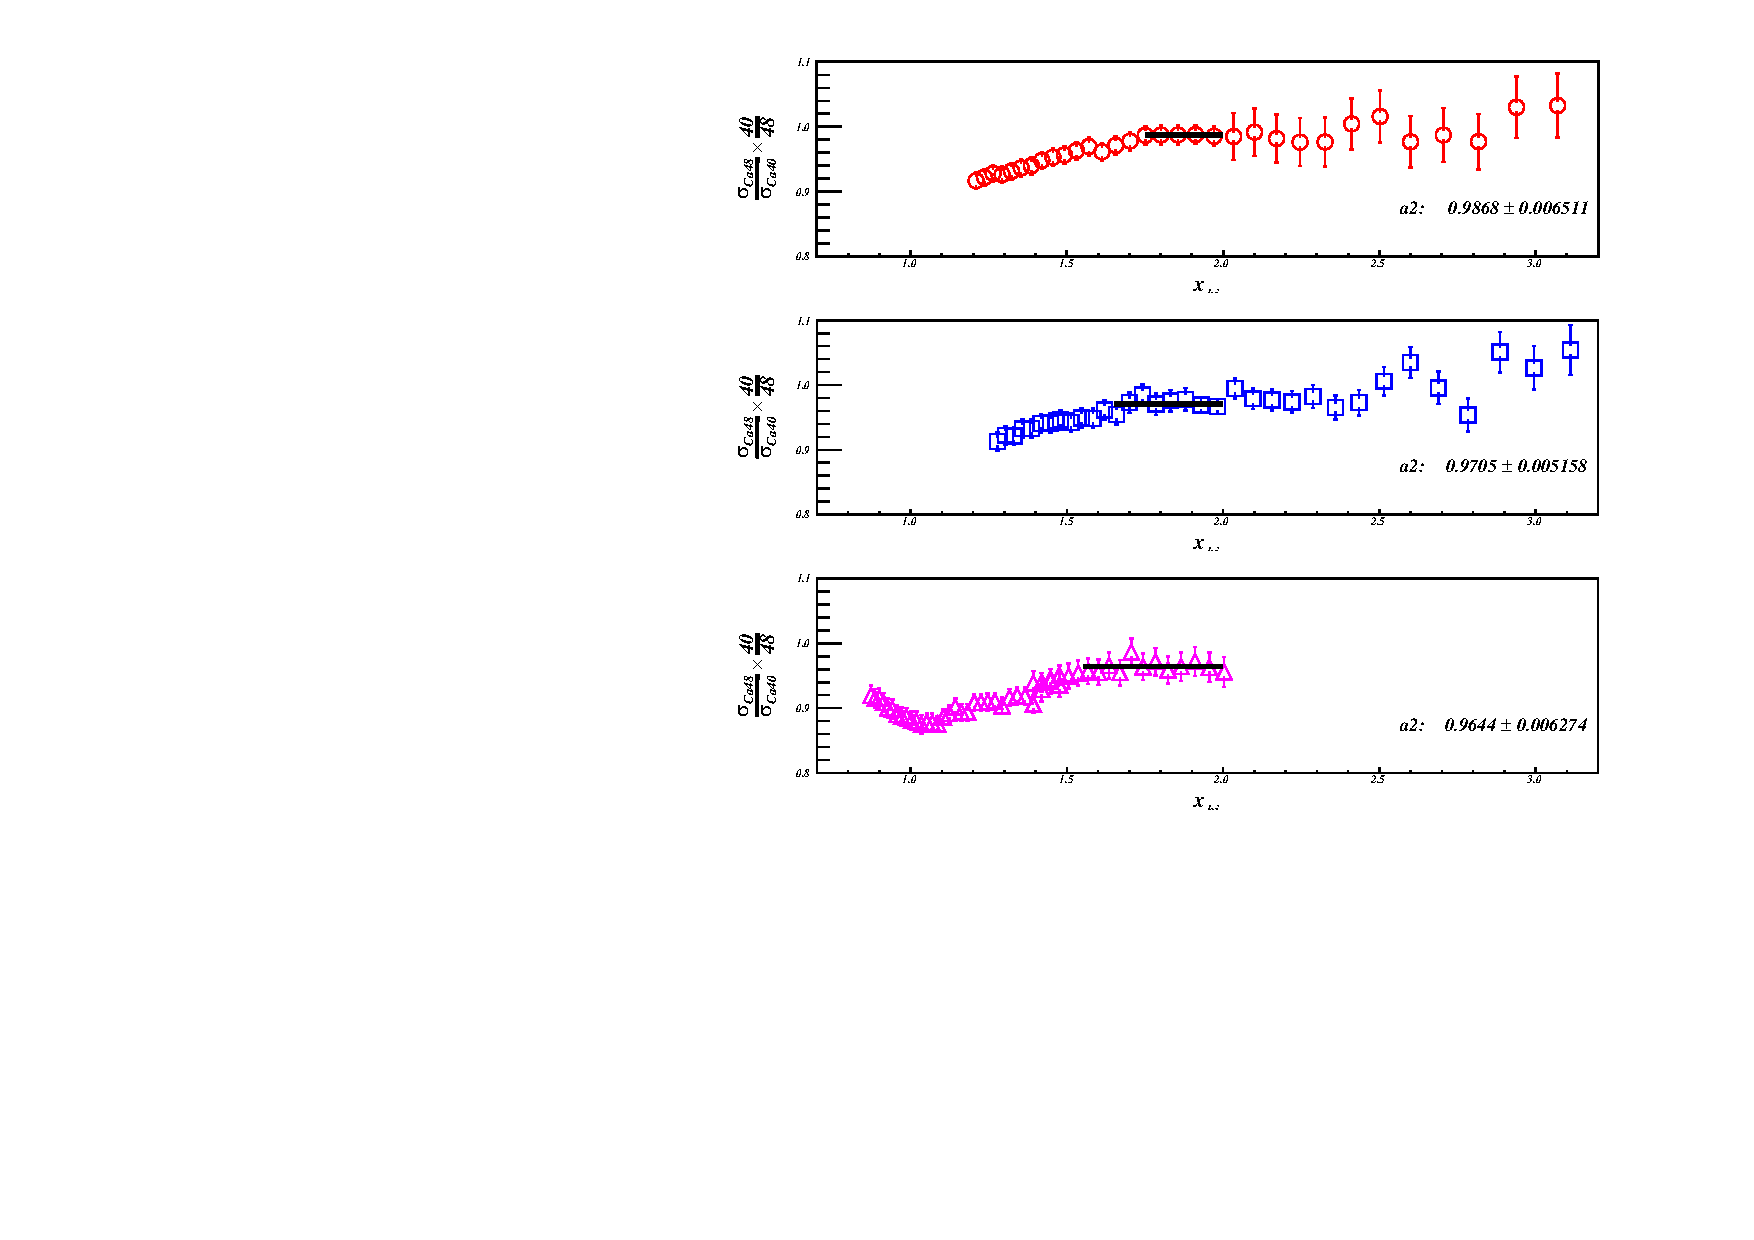
\includegraphics[type=pdf,ext=.pdf,read=.pdf,width=1.0\textwidth]{./figures/xs/Ca48_Ca40_XS_Ratio_Fit}
    \caption[Fitting of $\mathrm{^{48}Ca}$ to $\mathrm{^{40}Ca}$ cross section ratio]{\footnotesize{Fitting of $\mathrm{^{48}Ca}$ to $\mathrm{^{40}Ca}$ cross section ratio for each kinematic setting, where each plot gives the result of each setting. The values of $\mathrm{a_{2}}$ are given in these plots. The results show that $\mathrm{a_{2}}$ is different in each setting.}}
    \label{ratio_ca48_ca40_fit}
  \end{center}
\end{figure} 

 The preliminary cross section ratio of $\mathrm{^{48}Ca}$ to $\mathrm{^{40}Ca}$ is presented in Fig.~\ref{ratio_ca48_ca40}. The ratio in the 2N-SRC region, $R_{2N-SRC}$, is fitted individually in each setting, as shown in Fig.~\ref{ratio_ca48_ca40_fit}. The average value of the ratios for three kinematics settings is 0.973$\pm$0.017. Note that there is a 3\% decrease from the lowest $\mathrm{Q^{2}}$ setting at $21^{\circ}$ to the highest one at $25^{\circ}$.
    
\section{SRC vs. EMC}
  As discussed in Section 2.3, the SRC and the EMC effect have a strong connection. As shown in Fig.~\ref{emc_vs_src}, the 2N-SRC plateau ($a_{2}$) is plotted against the slope of the EMC effect, and for all measured nuclei, the plot reveals a nearly linear correlation. The preliminary $a_{2}$ value of $\mathrm{^{40}Ca}$ is included in the study of the correlation between the EMC and the SRC, as shown in Fig.~\ref{emc_vs_src_xgt2}. The new data point falls onto the linear fit and supports the conclusion that the EMC effect and the SRC are strongly connected. Note that the error bar of the new data point will be larger after including all systematic errors.
\begin{figure}[!ht]
  \begin{center}
    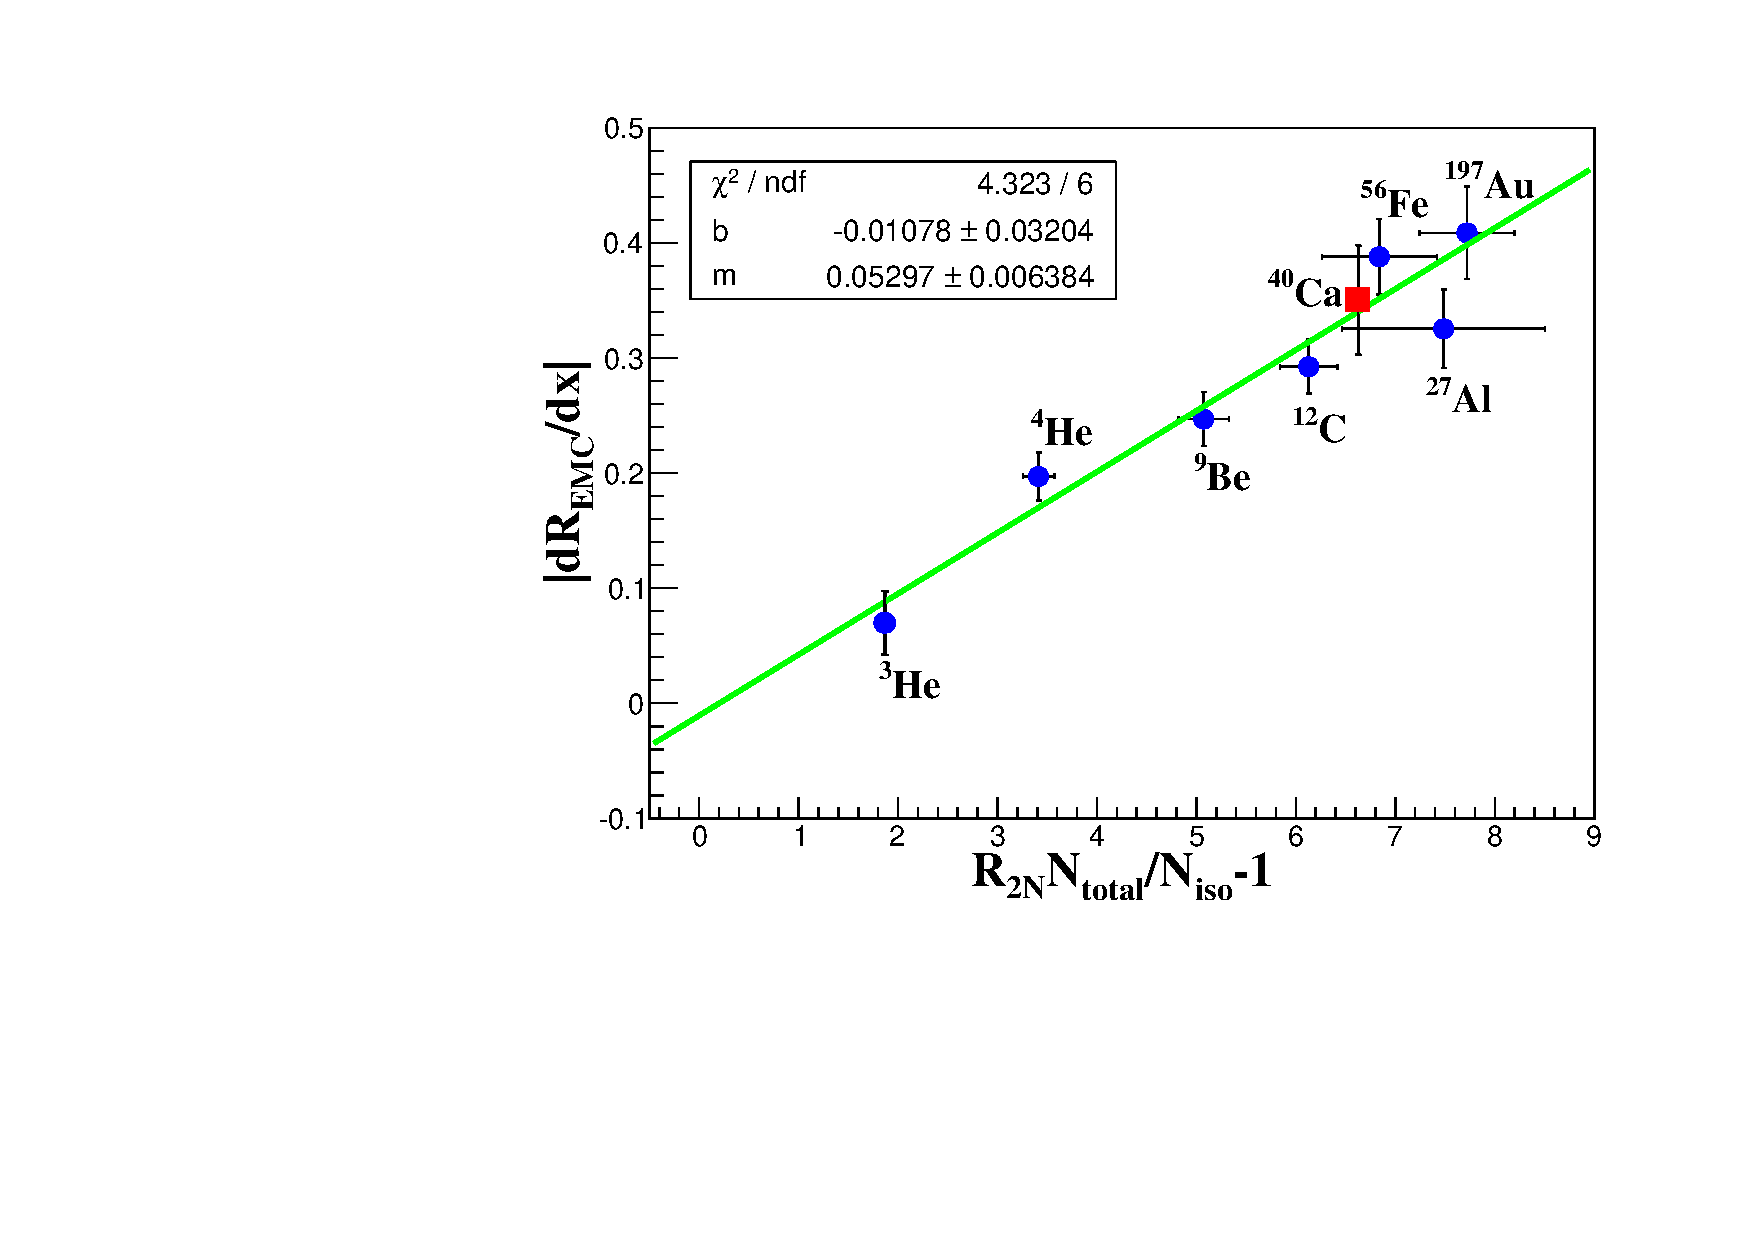
\includegraphics[type=pdf,ext=.pdf,read=.pdf,width=1.\textwidth]{./figures/xs/EMC_SRC_XGT2}
    \caption[EMC vs. SRC with the new $\mathrm{^{40}Ca}$ measurement]{\footnotesize{EMC vs. SRC with the new $\mathrm{^{40}Ca}$ measurement. In the x-axis, $N_{total}=A(A-1)/2$ and $N_{iso}=(A-Z) Z$.}}
    \label{emc_vs_src_xgt2}
  \end{center}
\end{figure}    

\section{Discussion}
 Before drawing conclusions by comparing the new results with results from previous experiments  and theoretical calculations, there are several aspects needed to be discussed.
 
   First of all, during the cross section extraction of each cryo-target, the aluminium events from the target cell's two endcaps were removed by cutting out the peaks of both endcaps in the $z_{react}$ distributions. However, due to the optics reconstruction and multi-scattering, there were still some aluminium events mixed with the events from the cryo-target. At low $x_{bj}$, the residual aluminium events are negligibly smaller compared with events from $\mathrm{^{2}H}$, $\mathrm{^{3}He}$ or $\mathrm{^{4}He}$. With $x_{bj}$ getting larger, the yields of the cryo-target decrease dramatically, but the aluminium yields reduce much more slowly. For example, when $x_{bj}$ approaches to 3, the $\mathrm{^{3}He}$ cross section drops quickly toward zero, so its yields may be comparable with the yields from the endcaps. A study of aluminium contamination for cryo-targets is being undertaken at this time.
  
 Secondly, the cross section models in XEMC require careful examinations for different nuclei.  As discussed in Appendix B, the QE cross section model is based on the y-scaling function which requires a clean subtraction of the DIS contribution. The DIS model used in this experiment has been updated but it still has to be tested. For $\mathrm{^{3}He}$, its cross sections drop off quickly to zero in the model when $x_{bj}$ approaches to 3, but in reality the cross sections should decrease more slowly. A special treatment must be applied to model this target. The cross section models of $\mathrm{^{40}Ca}$ and $\mathrm{^{48}Ca}$ were first developed in this experiment and iterated based on the new data. However, the models could not be compared with pre-existing data since these two targets were firstly measured in this experiment in such a high $\mathrm{Q^{2}}$ range. 
 
 Moreover, this experiment ran at lower $\mathrm{Q^{2}}$ settings and the data might include contamination from processes other than the SRC at large $x_{bj}$. As discussed in Section 2.2.1, in performing a clean study of the SRC at high $\mathrm{Q^{2}}$, it is essential to look beyond the mean field contribution and other competing processes. Meanwhile, the effect of FSI becomes more significant at low $\mathrm{Q^{2}}$ (Section 2.3). Hence, this experimental data may be contaminated by the contributions from the mean field processes and the FSI. It still requires more theoretical studies to better understand these effects.
  
 Last but not least, due to the non-uniform target densities, the radiative correction of cryo-targets is more complicated (see Appendix D). Meanwhile, the current cross section model uses the peak-approximation method to calculate the radiative effect on the simplified density distributions, as discussed in Section D.4. This method may underestimate the radiative effect at large $x_{bj}$, and has to be carefully examined by more sophisticated methods. 

\chapter{Conclusion and Perspective}
 The E08-014 studied the short-distance properties of the NN interactions in the region of $1.3<x_{bj}<3$ where two experiments~\cite{PhysRevLett.96.082501,PhysRevLett.108.092502} showed different results in the 3N-SRC region. The preliminary results presented in this thesis confirm the 2N-SRC plateau at $1.3<x_{bj}<2$ as observed by previous experiments, but indicated no 3N-SRC plateau under the current analysis. The preliminary result of the $\mathrm{^{48}Ca/^{40}Ca}$ ratio agrees with the A(e,e'pN) measurement~\cite{Subedi:2008zz} which claims that the tensor force leads to the dominance of $np$ pairs in the 2N-SRC. There were still several analysis tasks before publishing the final results. For example, the aluminium contamination in the cryo-targets and the radiative corrections, must be carefully studied.

 New experiments have been approved in Hall-A and Hall-C at JLab, to study the isospin dependence in the SRC~\cite{E12_11_112_pr}, map-out the SRC and the EMC effect for a wide range of nuclei in different kinematic regions~\cite{E12_10_103_pr,E12_06_105_pr,E12_10_008_pr,E12_11_107_pr,E12_10_003_pr}, and systematically study the linear connection between these two effects. The results from this experiment will provide an important input for new experiments and for future theoretical developments.
